% \documentclass[9pt,conference]{IEEEtran}
% \usepackage[utf8]{inputenc}
\documentclass[12pt]{article}
\usepackage[utf8]{inputenc}
\setlength{\parskip}{\baselineskip}
\setlength{\parindent}{0pt}
\usepackage{amsmath}
\usepackage{amssymb}
\usepackage{mathtools}
\usepackage{hyperref}
\usepackage{multirow}
\usepackage{floatrow}
\usepackage{float}
\usepackage{setspace}
\usepackage{tocloft}
\usepackage{caption}
\usepackage{subcaption}
\usepackage{titlepic}
\setlength{\cftbeforesecskip}{3pt} % for table of contents
\usepackage[a4paper,left=30mm,right=30mm]{geometry}

\title{\parbox{\linewidth}{\vspace{-7ex}\centering%
  
\includegraphics{PNGLogo.png}\vspace{5ex}\endgraf\bigskip\bigskip
  Interpretable Machine Learning for Time Series Data in an ICU Setting}}
\author{\parbox{\linewidth}{\centering%
  Gareth Booth\endgraf\bigskip\bigskip
  Supervised by Dr Sally Shrapnel}}
\date{\parbox{\linewidth}{\centering%
  Submitted for the degree of Bachelor of Engineering (Honours) for the School of ITEE\endgraf\bigskip\bigskip\today
  }}

\begin{document}

\maketitle
\newpage

\begin{flushright}
% 	ADDRESS LINE 1\\
% 	ADDRESS LINE 2\\
% 	Tel.\ (07) nnnn nnnn\\
% 	\medskip
% 	\today
\end{flushright}
\begin{flushleft}
  Prof Amin Abbosh \\
  Head of School\\
  School of Information Technology and Electrical Engineering\\
  The University of Queensland\\
  St Lucia, Q 4072\\
  \bigskip\bigskip
  Dear Professor Abbosh,
\end{flushleft}

In accordance with the requirements of the degree of Bachelor of
Engineering in the division of 
Electrical Engineering,
Electrical and Biomedical Engineering,
Electrical and Computer Engineering,
Software Engineering,
Mechatronic Engineering,
I present the
following thesis entitled ``Interpretable Machine Learning for Time Series Data in an ICU Setting''.  This work was performed under the supervision of
Dr Sally Shrapnel.

I declare that the work submitted in this thesis is my own, except as
acknowledged in the text and footnotes, and has not been previously
submitted for a degree at The University of Queensland or any other
institution.

\begin{flushright}
	Yours sincerely,\\
% 	\medskip
% 	\emph{Author's Signature}\\
	\medskip
	Gareth Booth.
\end{flushright}

\newpage

\section*{Acknowledgments}

I would like to acknowledge Sally Shrapnel for the time she spent advising my thesis and it's direction, and for introducing me to machine learning research in the first place. Thanks to Samuel Hinton, Kyle Young and Michael Kewming for creating some of the data processing code. 

\newpage
\section*{Abstract}

Health emergencies such as the current COVID-19 pandemic put great strain on ICU clinicians. Using machine learning to predict patient outcomes using time series ICU data seems to be a promising way to reduce information overload and help doctors better manage their patients. Using the MIMIC-III database, we create an ICU dataset of 2870 patients and evaluate it on an LSTM model to predict patient mortality, achieving an 87\% accuracy. We show that SHAP, a popular interpretability method, is able to create rich global explanations of this model, however is inadequate for local explanations over full time series. Modifications to the SHAP library are proposed to better handle local explanations, and these modifications are evaluated. This new SHAP is shown to provide local accuracy, but is unsuitable for global explanations. For validation, the accuracy and explanations from the LSTM are compared with those of random forests trained on fixed amounts of admission and final day data.

\newpage
\tableofcontents
\newpage
\section{Introduction}
Health emergencies such as pandemics cause great strain to the healthcare system and create a shortage of intensive care unit (ICU) beds. During these emergencies, many hospitals gather data from their patients in ICU including vital signs, procedures and diagnoses. This data could be used to inform doctors about effective treatments or provide early warnings. However, there is often an information overload for ICU specialists, considering the number of patients, the time each patient spends in ICU and the number of measurements taken \cite{KajiLSTM}.

As machine learning requires a large amount of data, it has great potential in this field. Recently, there have been a large number of studies released in this area. Some of the problems that these studies focus on include predicting clinical events such as death, myocardial infarction or discharge \cite{KajiLSTM}. 

There are a few factors that make this a challenging domain. While there is a relatively large amount of open access data available compared to other fields, it can be challenging to process. Also, the time series nature of ICU data limits the choice of machine learning models substantially. 

Few studies incorporate explainability techniques. Machine learning models normally give a single output, which is a prediction for the given data. This does not given any explanation as to why that prediction might be true. Explainability (or interpretability) techniques allow seeing which features are important for a prediction, and can help give users of the model confidence \cite{YoungKyle2019Dnno}.

One use of explainability is to recognize biases. Machine learning models are capable of learning very complex relationships, and if a dataset contains a bias, the model is likely to also learn this bias. Searching the dataset manually for biases is not feasible, due to the amount of data and the presence of unknown biases \cite{YoungKyle2019Dnno}. Explainability techniques can reveal these biases by highlighting spurious relationships, which domain experts can identify.

The importance of ICU data has been highlighted in the ongoing COVID-19 pandemic. One possible application of this work is to perform transfer learning to a new dataset with  data from COVID-19 patients. Interpretability techniques can highlight relationships between features, which could potentially reveal novel insights which could be used by doctors. Another possible application of robust explainability techniques for time series data is to sanity check existing models. This can be possible for some model agnostic techniques.

The key question of this thesis is if it's possible to predict death using time series ICU data in an interpretable way.

\section{Background}
%too much overlap with proposal?

\subsection{Machine Learning on ICU Data}
\label{Machine Learning on ICU Data}
The first difficulty arising from using ICU data is the nature of the time series data. Time series data is 3 dimensional. Specifically, an ICU dataset will have many patients, each with many features (e.g. vital signs) over many different points in time (e.g. every hour). Time series machine learning models should be able to handle any length of time series. This means the model should take inputs of the shape $(x,y,z)$ where $x$ and $y$ are any length, and $z$ is the number of features which is fixed. The model will output a list of predictions, one predictions for each $x$.

One of the problems that we can ask using this time series data is given a patients data, predict if this patient was discharged or died, where discharged means discharged from ICU alive. However, this problem means that the machine learning model could be looking at the final point of data to make a prediction, i.e. the data just before the patient died. Care needs to be taken to ensure that the model is not only using this data. Another related problem is of predicting 90-day mortality, which is an easier problem \cite{ICUFancyLSTM}.

A machine learning model to predict ICU death could be useful in practice to find out if a patient is going to die soon. If the model predicts that the patient will die given the current data, then extra care can be given to them. If the model predicts that the patient will be discharged soon, then other patients can be prioritized.

Another way of using ICU data is to make predictions using a fixed amount of data, e.g. only admission data. Data from the first $n$ days can be used, but $n$ must be known before the model has been created. This problem is suitable for traditional machine learning models. These models can handle 2 dimensional data, i.e. many data points with many features. These models will output 1 prediction for each data point (where a data point is a single set of features). Similarly, data from the last $n$ days of a patients ICU stay can be used instead. However, due to these models using less data to make predictions, it is reasonable to expect these models do not have as much predictive power as a time series model. \cite{KajiLSTM,ICUFancyLSTM} find that models benefit from access to longer time series data.

One of the most widely used ICU datasets is MIMIC-III, a dataset of deidentified data from 53,423 distinct hospital admissions \cite{MIMICIIIdatabase}. Due to its size and public availability, it has been widely used for benchmarking machine learning tasks. The data includes bio-markers, drug administrations, procedures and diagnoses (using International Classification of Diseases).

Most studies using time series data use a fixed temporal resolution, for example 1 day in \cite{KajiLSTM} and 1 hour in \cite{ICUFancyLSTM}. However, some techniques exist to handle continuous data \cite{GRUODE}.

\subsection{LSTMs}
Recurrent neural networks (RNNs) are neural networks with a feedback loop \cite{ColahLSTM}. An RNN consists of a neural network that takes and outputs some data, but also takes some state from the previous application of the neural network as input. This means that an RNN is able to make predictions based on what it's seen before, and is also able to handle an arbitrary length of input sequence.

Long short-term memory (LSTM) is an RNN architecture that achieves greater performance than a traditional RNN. It allows models to learn long-term dependencies, i.e. information from many inputs ago \cite{ColahLSTM}. LSTMs take two inputs from the previous application, one is called the ``cell state'' and the other is the previous output vector. This extra cell state is updated each application by removing unimportant data and adding new relevant data from the current input. 

The below figure shows an example of an LSTM network. Here, the network has been unravelled for demonstration, but the different inputs are applied to exactly the same  model. The top `line' represents the cell state, which is modified by the original input and the bottom `line' is the output from the model at that time step. It is important to note that the size of the vectors passed on through the model is a hyper-parameter of this model.

\begin{figure}[H]
\centering\caption{Example LSTM network \cite{ColahLSTM}}
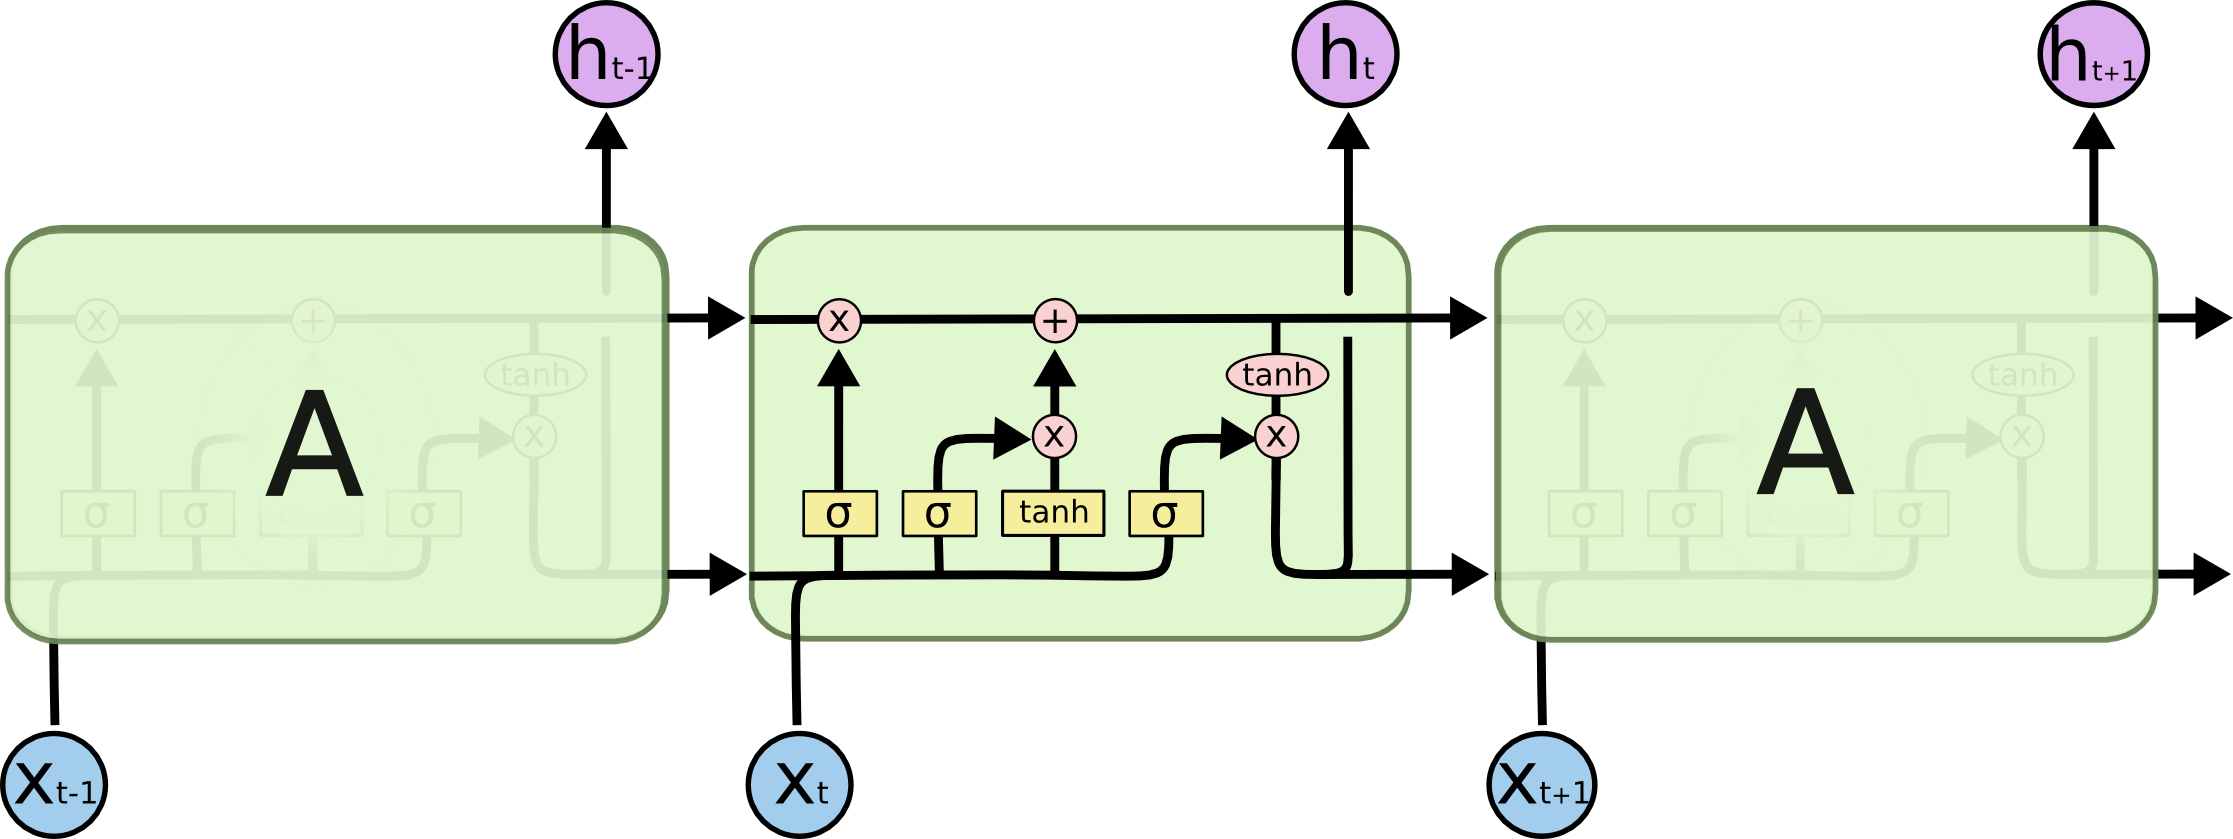
\includegraphics[scale=0.5]{LSTM3-chain.png}
\label{Example LSTM}
\end{figure}

An example of an LSTM used with ICU data to predict mortality is in \cite{ICUFancyLSTM}. They use a vanilla LSTM with hyperparameter training. Their model achieves an AUCROC of 0.88, however their dataset is not publicly available and uses a very high temporal resolution of 1 hour.

\subsection{Random Forests}
There are many machine learning models that handle a fixed amount of input data. LSTMs can be made to handle fixed amounts of data by limiting the length of input sequences when defining the model. 
Random forests are a popular type of model. Random forests (RF) and gradient boosted trees achieve state of the art performance in many domains, particularly when features are individually meaningful and in tabular form \cite{TreeExplainer}. Random Forests involve ensembling many decision trees and getting a single aggregated result. Gradient boosting methods are slightly different in the way they're constructed.

Mortality is predicted in patients with unplanned extubation in \cite{CompareFourML}. The paper compares the performance of four different machine learning architectures, including neural networks, logistic regression models and random forests. The study concluded that random forests were the most suitable for this task, having the highest AUROC, precision and recall. However, the dataset only contains data from 341 patients in this study, and cannot be used as a benchmark as it does not use the MIMIC-III database. 

\subsection{SHAP}
\label{SHAP Intro}
SHAP is a model agnostic, local interpretability method \cite{SHAP}. It is a unification of six existing methods, and outputs the importance value for each feature based on the contribution that feature makes to the prediction. It is based on Shapley values from co-operative game theory, and has a strong theoretical justification \cite{YoungKyle2019Dnno,ICUFancyLSTM}. The SHAP value for a feature is it's compound effect when interacting with all other features. A positive value means the feature moves the prediction in the positive direction. For example, if the model outputs 1 for death, then a positive value represents an increased risk of death \cite{SHAPInteraction}.

SHAP is used in \cite{ICUFancyLSTM} to tell if a given feature increases or decreases the probability of mortality. It is used to show that, for example, the presence of a small age in a patient greatly decreases risk, while a higher age increases it. 

As an example application of SHAP, consider a model predicting mortality trained on an ICU database \cite{SHAPInteraction}. The below figure shows the effect of systolic blood pressure. Each dot represents one point of data input to the model. For each point, a SHAP value is calculated ($y$-axis). This shows that SHAP is able to find complex relationships, such as how lower systolic blood pressure generally decreases the patients risk of death, however a sufficiently low value will again increase the patients risk. Also, SHAP shows how age affects systolic blood pressure, which can be seen by the colour of the points. 

\begin{figure}[H]
\centering\caption{Example SHAP application from \cite{SHAPInteraction}}
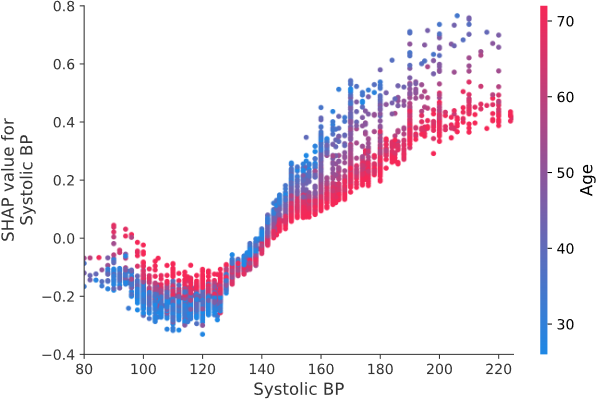
\includegraphics[scale=0.7]{SHAP example.png}
\label{SHAP Example Systolic BP}
\end{figure}
The local explanations from SHAP can be combined to make global explanations \cite{TreeExplainer}, as the above figure shows from plotting all local explanations. Further global explanations can be found by taking the mean absolute SHAP value of all features, which allows the comparison of model sensitivity between all features \cite{molnar2019}.

An enhanced version of SHAP for random forests is introduced in \cite{TreeExplainer} and \cite{SHAPInteraction}. This includes the ability to calculate interaction values between features. This can allow quantifying which features interact the most. As an example, the above figure shows that age and systolic blood pressure interact strongly.

Unfortunately, there is no support in the framework for time series data. Using vanilla SHAP in a time series data setting involves flattening the 3 dimensional time series data to 2 dimensions by removing the time dimension. 

\subsection{Project Overview}

This investigation has been broken down into three parts. 

Firstly, a time-series ICU dataset for this project must be created. This will involve processing the freely available MIMIC-III database, and careful feature selection in order to provide sufficient prediction power and enough data points for machine learning. 

Next, two different architectures of machine learning models will be trained on this dataset. This will include an LSTM model trained on time series data, and random forests trained on admission and final data. The results from these models will be evaluated and compared. 

Finally, interpretability methods will be investigated. Vanilla SHAP on the LSTM will be investigated, and a new modified version of SHAP designed for time series data will be proposed. These explanations will be compared to those of the random forest when using TreeExplainer. 

\section{Data Processing}

The first state of the project is to investigate the available data and create a suitable dataset. 

The use of daily data was chosen early in the project. The initial plan as outlined in the project proposal was to create a dataset from MIMIC-III that resembles a COVID-19 dataset which used daily data. However, insufficient data was obtained for this new dataset and this line of investigation was cancelled.

The Python programming language was chosen due to it being the de facto standard for machine learning. Pandas \cite{pandas} was chosen to manipulate the data due to previous experience with the framework, and matplotlib \cite{matplotlib} was used to visualize the results for the same reason. 

\subsection{MIMIC-III}

MIMIC-III consists of data from two different ICU database systems, CareVue and Metavision. There are 57,272 unique hospital admissions. The raw data is a series of csv files of database tables, as is documented in \cite{MIMICIIIdatabase}. The tables of interest for this study include CHARTEVENTS and D\_ITEMS.

CHARTEVENTS contains a list of events, also called charted data or measurements. In this table, the key columns are HADM\_ID, which is a unique ID given to hospital patients for a single admission. CHARTTIME gives the time of the event, ITEMID gives the ID of the event and VALUE gives the value of the event. In total, there are 330,712,483 rows in the chartevents table.

D\_ITEMS contains the definition of all ITEMIDs in the CHARTEVENTS table. There are 6463 unique items, i.e. 6463 different types of measurements. The below table shows 12 of the most common items in the CHARTEVENTS table, with the Item Name from the D\_ITEMS table.

Note the two different ``Heart Rate" features and oxygen saturation. These are from the different ICU databases (the lower ITEMIDs are always from CareVue).

\begin{center}
\captionsetup{type=table}
\begin{tabular}{|l|l|l|ll}
\cline{1-3}
ITEMID & Count   & Item Name                   &  &  \\ \cline{1-3}
211    & 5180809 & Heart Rate                  &  &  \\ \cline{1-3}
742    & 3464326 & calprevflg                  &  &  \\ \cline{1-3}
646    & 3418917 & SpO2                        &  &  \\ \cline{1-3}
618    & 3386719 & Respiratory Rate            &  &  \\ \cline{1-3}
212    & 3303151 & Heart Rhythm                &  &  \\ \cline{1-3}
161    & 3236350 & Ectopy Type                 &  &  \\ \cline{1-3}
128    & 3216866 & Code Status                 &  &  \\ \cline{1-3}
550    & 3205052 & Precautions                 &  &  \\ \cline{1-3}
1125   & 2955851 & Service Type                &  &  \\ \cline{1-3}
220045 & 2762225 & Heart Rate                  &  &  \\ \cline{1-3}
220210 & 2737105 & Respiratory Rate            &  &  \\ \cline{1-3}
220277 & 2671816 & O2 saturation pulseoxymetry &  &  \\ \cline{1-3}
\end{tabular}
\captionof{table}{Most Common Items}
\label{Most Common Items}
\end{center}

The below figure shows the occurrences for the 300 most commonly appearing items. 
\begin{figure}[H]
\centering\caption{Number of Data Points for Most Common Items}
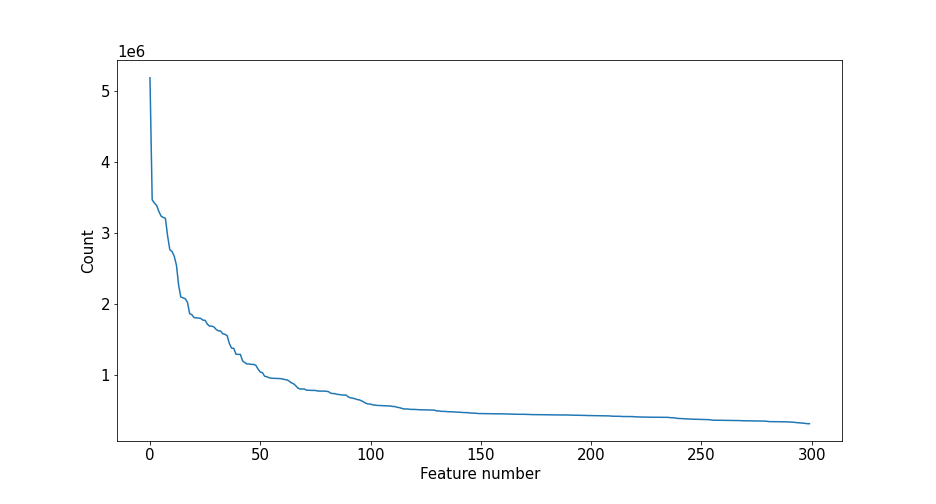
\includegraphics[scale=0.45]{Number of Data Points for Most Common Items.png}
\label{Number of Data Points for Most Common Items)}
\end{figure}

While there is a lot of data available in MIMIC-III, unfortunately a significant amount of it cannot be used in this study. This is due to the nature of the problem where we are using daily data, meaning only 1 record can remain for each feature for each patient for each day.  All data points from the same day for the same feature for the same patient are dropped except for the first element found in the dataset. Using only 1 point per day has a significant effect on the amount of available data, and also introduces the problem of missing data.

The below table shows how the count is affected. Counts now represent the number of measurements when there can only be 1 measurement per day per patient. The number of measurements for the top item has decreased by an order of magnitude. Also, all Metavision items are no longer present in the most common list, in fact there are no Metavision items in the top 90 most common elements. This suggests that the Metavision data is of a higher temporal resolution, and that a higher temporal dataset may be possible using this subset of MIMIC-III.

\begin{center}
\captionsetup{type=table}
\begin{tabular}{|l|l|l|}
\hline
ITEMID & Count  & Item Name           \\ \hline
211    & 241092 & Heart Rate          \\ \hline
31     & 236115 & Activity            \\ \hline
80     & 230807 & Bowel Sounds        \\ \hline
212    & 157814 & Heart Rhythm        \\ \hline
742    & 157746 & calprevflg          \\ \hline
161    & 157608 & Ectopy Type         \\ \hline
618    & 157423 & Respiratory Rate    \\ \hline
646    & 157363 & SpO2                \\ \hline
432    & 157020 & Level of Conscious  \\ \hline
617    & 156824 & Respiratory Pattern \\ \hline
\end{tabular}
\captionof{table}{Most Common Items (Once per Day per Patient)}
\label{Most Common Items (Once per Day per Patient)}
\end{center}

The below figure is analogous to Figure \ref{Number of Data Points for Most Common Items)} except for the new data restriction. Clearly, there is much less data available for this kind of problem in general, which is a challenge in the ICU data setting.

\begin{figure}[H]
\centering\caption{Number of Data Points (Once Per Day per Patient)}
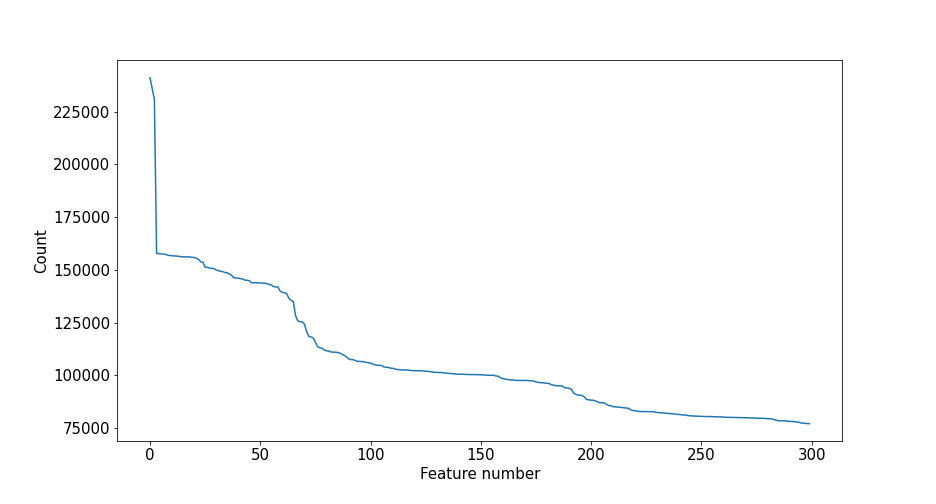
\includegraphics[scale=0.45]{Number of Data Points (Once Per Day per Patient).png}
\end{figure}

\subsection{Feature Selection and Missingness}

In order to create a usable dataset, features must be judiciously chosen. There is a trade off between getting enough relevant features and getting enough data, as too many features will mean too many features are empty. This can be demonstrated by the figure below.

\begin{figure}[H]
\centering\caption{Days of Full Data}
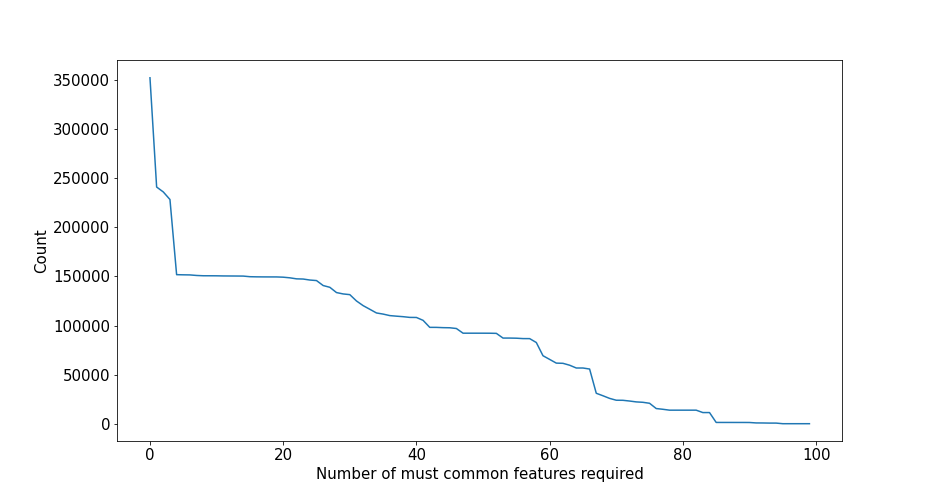
\includegraphics[scale=0.45]{Days of Full Data.png}
\end{figure}

The $y$-axis represents the number of full days of data, and the $x$-axis is the number of the most commonly appearing features used. For example, the point (3, 228383) means that if you want to make a dataset using the 3 most common features (see Table \ref{Most Common Items (Once per Day per Patient)} to see these features), you will have 228383 days of data. Patient days with any missing data features are not included. The point (0, 352325) shows that there are 352325 different combinations of days and patients in the database.

While this may look like a large amount of data, a lot of these features are not useful or not documented. For example, there is a ``Temperature F'' and ``Temperature C (calc)'' field. Also, units of measurement in CareVue are not always specified. There are three different items that all represent oxygen saturation in the top 26 most common ITEMIDs. 

In order to maximize the number of records obtained, it is important to use both databases and all duplicated fields. This involves finding, for a single feature, all ITEMIDs that represent that feature from both databases. This was done for a series of features that were thought to be of clinical significance and features that contain a significant number of records, e.g. some of those in the above tables. This list of features can be found in the file `variables.csv' in the repository (See Appendix A).

After this, a subset of these features needed to be chosen that satisfied a few criteria. After dropping all days with missing data, there had to be enough records overall to perform machine learning, which in general is at least 5000 data points \cite{5000Points}. Also, there needed to be a high ratio of patient mortality in this subset to avoid a class imbalance problem, which always provides a challenge for machine learning. Finally, there needed to be enough data on the day of the outcome.

Demographic features such as the patients weight and height are only recorded once during the hospital stay, and so care must be taken to propagate them to all rows for each patient.

Feature selection involved choosing features that resulted in a significant amount of records remaining from this initial subset of clinically relevant features. The final numeric features chosen are as follows: Creatinine, HCO3, Heart rate, haemoglobin, platelet count, potassium, respiratory rate, sodium, weight, SaO2. 

More important features for performing machine learning are included. HADM\_ID is a hospital admission ID, which is needed to uniquely identify sequences and is used as a patient ID. Each day of data also has a CHARTDATE, and a DAYS\_TO\_DISCH, and the day relative to the start of their ICU stay. The patient's age, gender and a boolean flag for death is also added.

As well as the above features, comorbidities can also be strong predictors of mortality. The following commodities were found in MIMIC from looking at ICD-9 codes in the DIAGNOSES\_ICD table: Chronic kidney disease, obesity, heart disease, asthma. The corresponding ICD-9 codes can be found in the `get\_all\_diagnoses' function in `process\_mimic.py' (See Appendix A). 

The next step of data processing is ensuring that, for each hospital admission, the ``final day" of data is complete, i.e. the day before discharge or death. However, the other days in a patients stay are not required. For example, a patient who has a stay of two weeks can have any days missing except for the final day. This requirement was done because of how critical the final days data is to this project. However it comes at a cost, as this single step decreases the number of hospital admissions in the data set from 21443 to 2935. Combining this with requiring a complete sequence removes too much data, and so isn't done. 

Finally, outliers are removed by removing all rows with data points having a z-score $>$ 4. This is done to remove very extreme outliers, which were most likely problems with data entry or incorrect units of measurement.

After processing, this data is saved in a flat file csv. 

\subsection{Final Dataset}

After the data processing, there are 2870 unique patient admissions. This represents a total of 15097 days of complete data, with 21 features.

The below figure shows the length of each patients' ICU stays. Clearly, most of the data in the dataset is from single day hospital admissions. Also, is it clear that the distribution between patients who died and patients who survived is different, and patients who died had a longer hospital stay on average (12.1 days compared to  9.3 days).

\begin{figure}[H]
\centering\caption{Number of Outcomes at Each Day}
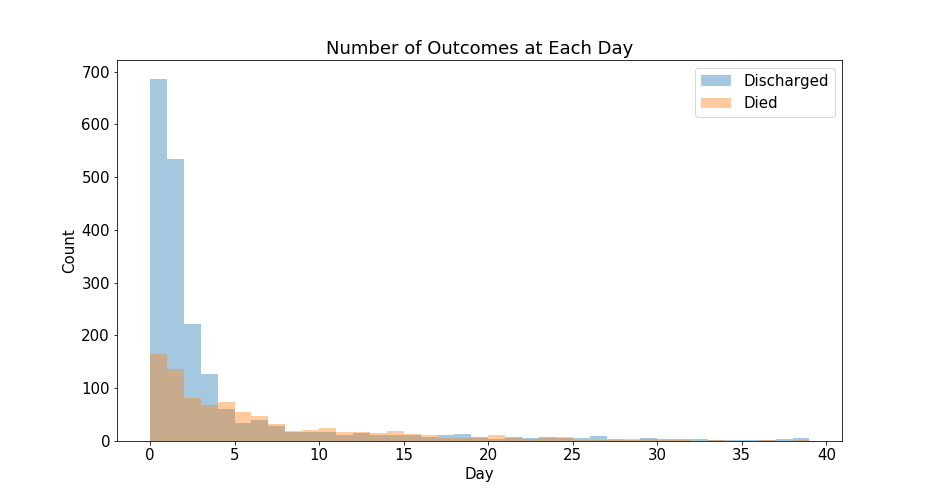
\includegraphics[scale=0.45]{Number of Outcomes at Each Day.png}
\end{figure}
The below figure shows the number of data points at each day. Day 1 has more data available than day 0 because many patients do not have complete admission data available. For the purposes of this study, admission data is data from the first day in the sequence. This figure shows that there are a significant number of data points at later days, for example there are 431 patients with an ICU stay longer than or exactly 10 days.

\begin{figure}[H]
\centering\caption{Number of Data Points for each Day}
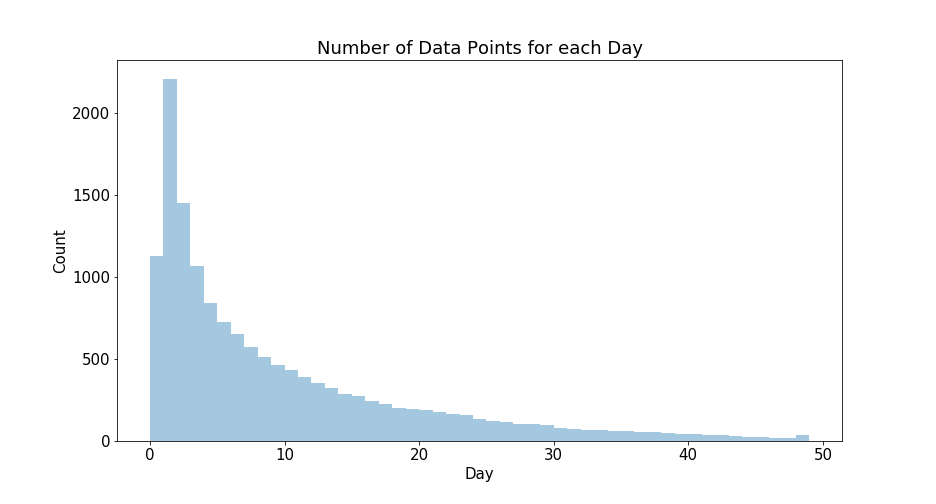
\includegraphics[scale=0.45]{Number of Data Points for each Day.png}
\end{figure}
The imbalance between discharge and death is large. Out of all 2870 patients, 1977 were discharged alive while 893 died. Discharged patients represent 68.8\% of the population. Therefore, an accuracy of 68.8\% could be achieved through guessing discharge. This number will form a minimum baseline for prediction accuracy. Note that the mortality in this subset is much higher than the in-hospital mortality rate of 11.5\% in the MIMIC-III study \cite{MIMICIIIdatabase}. 

Below is a correlation matrix, showing all features used for prediction, as well as ``DEATH'', which is the target feature. Some obvious correlations are highlighted, such as between obesity and weight, gender and weight, and some medically significant relationships such as chronic kidney disease and creatinine, sodium and HCO3 and others such as age and death.

\begin{figure}[H]
\centering\caption{Correlation Matrix}
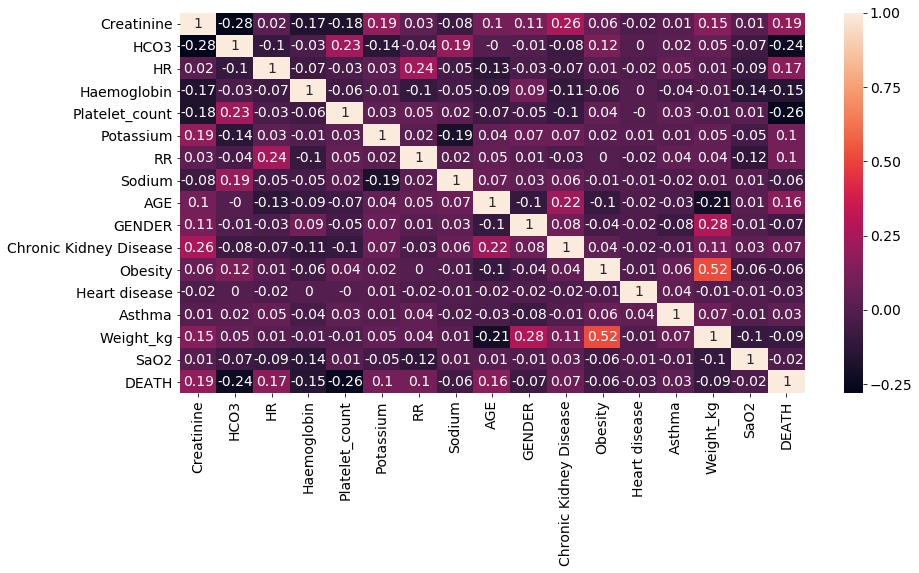
\includegraphics[scale=0.45]{Correlation Matrix.png}
\end{figure}

An example histogram of Heart rate is shown below. The distribution of heart rate between death and discharge appear to be different. Histograms for all features can be found in the notebook `MIMIC death.ipynb' (See Appendix A).

\begin{figure}[H]
\centering\caption{Histogram for Heart Rate}
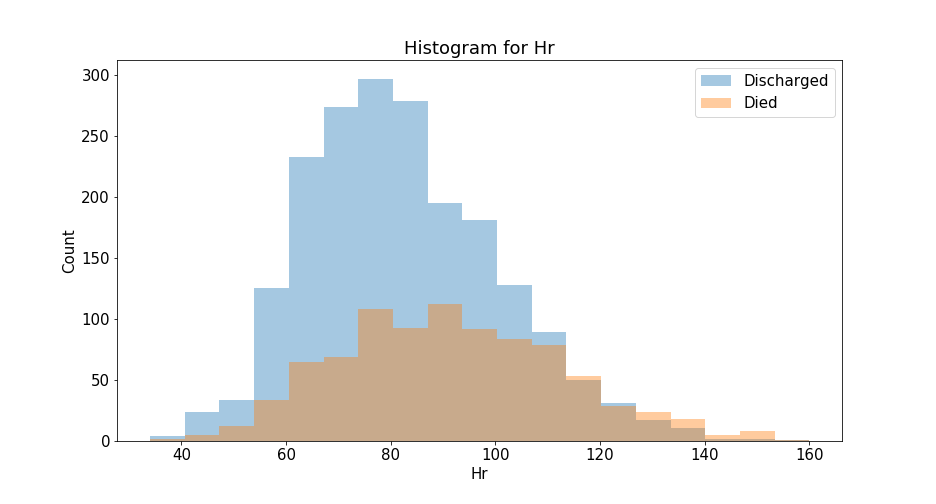
\includegraphics[scale=0.45]{Histogram for Hr.png}
\end{figure}

Code for this section is in the repository under the `mimic' folder which contains the python file `process\_mimic.py'. The dataset is created in the notebook `MIMIC dataset.ipynb'. (See Appendix A)

\section{Classifier}
% \subsection{Motivation}

Two different types of machine learning models are used. LSTMs are used because they operate on time series data, which is the key focus of this investigation. LSTMs will be trained on the time series data and evaluated. 

However, random forests will also be used, even though they do not operate on time series data. They are used instead to validate the LSTM. Care must be taken to ensure the LSTM is actually exploiting the time series nature of the data, and not just using the final day of data to make a prediction (i.e. the day of discharge or death). To help test if this is the case, a random forest can be trained on the last day of data. If the accuracy of the random forest is worse than the LSTM, then it is reasonable to conclude that the LSTM is using more than the last day of data since random forests represent the state of the art for such classification. 

Random forests will also be trained on admission data as this is a popular problem in this space, and a large difference in accuracy between admission only data and LSTMs helps motivate the use of time series data. 

Also, random forests with varying amounts of data will be trained. For example, a random forest will be trained with access to the first N days. This will be done to investigate an alternative problem where a fixed amount of data is known, in which case an LSTM may not be required. 

\subsection{Model Building \& Results}

Firstly, for model training and evaluation, a 20\% split test and train set was created. The training set contains 2296 admissions and 12310 days of data, while the test set has the remaining 574 admissions and 2787 days. This same dataset split will be used for both different types of models. 

\subsubsection{Random Forest}
XGBoost is chosen as the random forest framework \cite{XGBoost}. This is a popular gradient boosted method. 

The first random forest experiment is to use admission data. Various lengths of admission data is used. For example, 1 day admission means only the information from the first day is used, 2 day admission means data from the first two days is used, etc. Note that for $n$ day admission data, ICU stays that are less than $n$ in length cannot be used. Therefore, increasing the number of days will decrease the data available. The below figure shows this.

\begin{figure}[H]
\centering\caption{Random Forest Admission Data}
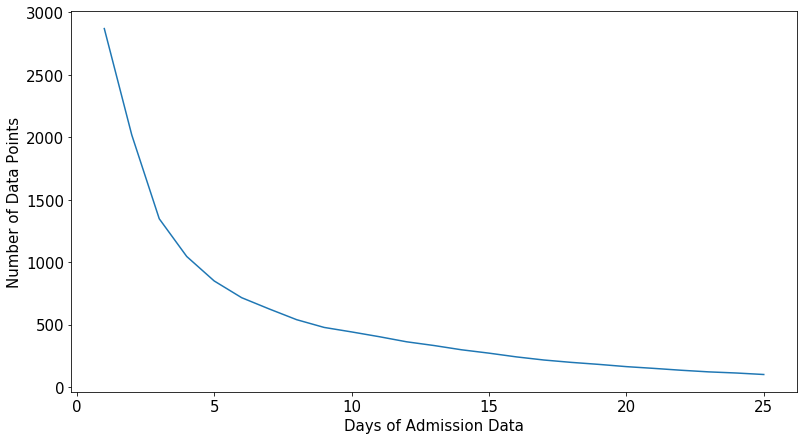
\includegraphics[scale=0.45]{Random Forest Admission Data.png}
\label{Random Forest Admission Data}
\end{figure}

Hyper-parameter grid search was done using  scikit-learn's GridSearchCV function \cite{scikit-learn}. The parameter ranges were: max\_depth from 3 to 10, alpha from 1 to 19, subsample from 0.1 to 1, colsample\_bytree from 0.1 to 1. The optimal values for these parameters are: max\_depth of 8, alpha of 9, subsample of 1, colsample\_bytree of 0.4. Max\_depth was later changed to 5 to reduce overfitting. Other parameters chosen are: learning\_rate of 0.05 and n\_estimators of 1000. This grid search was done on 2 days of admission data. Class weighting is used.

For each different number of days of data, the model is recreated and trained. This must be done since the random forest cannot take a varying amounts of data. Also, a 20\% holdout test set is created for each different length and the model is evaluated on this. The `discharged' and `death' lines in the below figure show the percentage of patients who were discharged alive and the percentage of patients who died in the dataset. The maximum of these two lines represent the baseline accuracy for the model. 

\begin{figure}[H]
\centering\caption{Random Forest Admission}
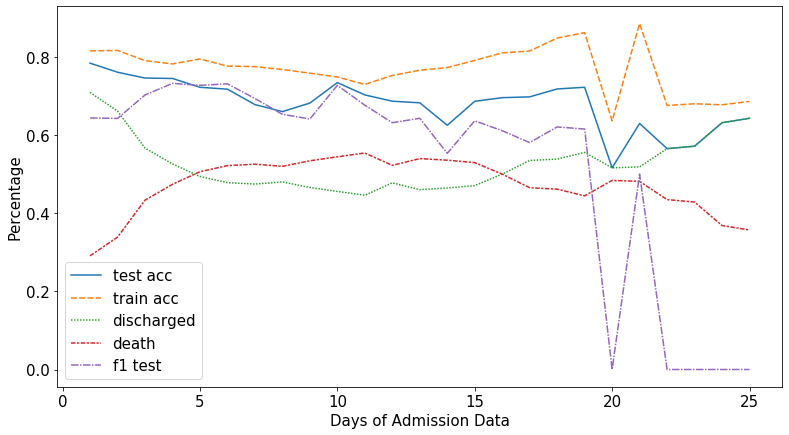
\includegraphics[scale=0.45]{Random Forest Admission.png}
\label{Random Forest Admission}
\end{figure}
The above figure shows the random forests performance as the number of days of admission data increases. 

The f1 score for the death class on the test set is also featured in the above figure. The f1 score shows how a model performs on an individual class, and is calculated using the precision and recall of that class. The f1 score for death is very low for the first few days of data when compared to the accuracy, suggesting the model is much better at predicting if the patient discharged successfully. However, as the death and discharge percentage approach 50\%, the f1 score begins to converge on the test accuracy, meaning both classes performed equally. %This shows the difficulty of dealing with class imbalance problems.

The random forests are able to generalize well while there is a large amount of data, such as in the first 5 days (see Figures \ref{Random Forest Admission Data} and \ref{Random Forest Admission}). However, the model does not generalize well past a certain point. For example, with 1 week of data the test accuracy becomes much lower than the train accuracy. When there is 20 days of admission data, the f1 score for the test set becomes zero (same for the train set). This means the model is always predicting discharge, since it is the most prevalent class. This is due to the small number of records available for these long sequences, which causes the random forests to be unable to learn meaningful relationships.

The next experiment tests a similar problem, where instead of admission data you are given data from the days before the outcome. The experiment is repeated exactly as before, except the $x$-axis is now the number of days of data before the final outcome.

\begin{figure}[H]
\centering\caption{Random Forest Discharge}
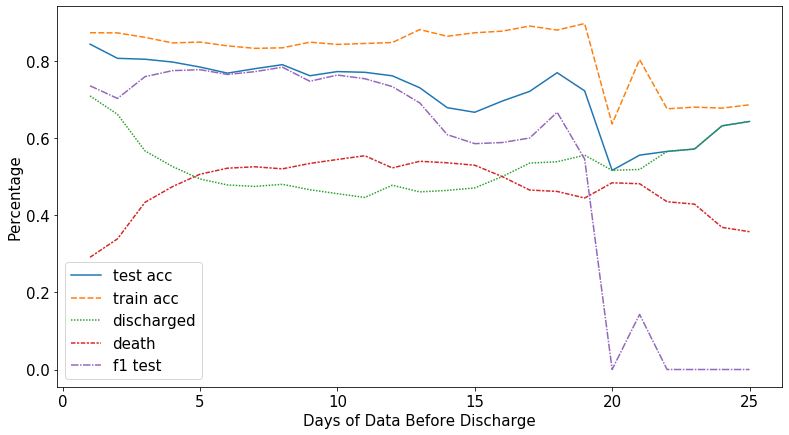
\includegraphics[scale=0.45]{Random Forest Discharge.png}
\label{Random Forest Discharge}
\end{figure}
Note that these random forest models attain significantly higher accuracy when compared to the admission models. For example, the 1 day admission data model accuracy is 78\%, while the 1 day discharge data is 84\%.

% TODO sample confusion matricies of 1 day for both of thesse?

Code for these experiments can be found in the `MIMIC death RF' notebook. 

\subsubsection{LSTM}
\label{LSTM}
Keras with a Tensorflow backend is chosen as the framework to create this model \cite{keras}. Keras is uesd due to its ease of use and contains a built in implementation of an LSTM. The keras functional API allows creating a complete machine learning model by building up layers of functionality \cite{keras}. This API can also accommodate multiple inputs and outputs in a single model. 

The base functionality of the LSTM model used in this study is very simple. First, it consists of an input layer. In order for the model to be able to handle arbitrary length time series, the input shape should be (?, ?, num\_features), where ? is an unspecified length and num\_features is the number of features in the data, which is 16 in this case (when using the notation from Section \ref{Machine Learning on ICU Data}). Next, a masking layer is added which masks out time steps where all features are zero. This is done so 3D numpy arrays arrays can be used, since 3d arrays require all dimensions to be known when they are created so all time series must be padded to the same length. It was verified that no actual data involved all features being zero before this step.

An LSTM layer is added next. This layer takes a 3D input from the previous layer and outputs a 2D output. It outputs a vector of length $n$ for each sequence, where $n$ is a hyper parameter of this model. This is connected to a hidden dense layer. Finally, a sigmoid dense layer is added to create a final numerical output between 0 and 1. A diagram of this model with 16 features and 128 chosen as the LSTM and hidden layer hyper-parameter is below. As is standard for binary classification, binary cross-entropy loss is used. All other parameters are left as their defaults from the Keras library \cite{keras}.

\begin{figure}[H]
\centering\caption{LSTM Model Diagram with Hidden Dense Layer}
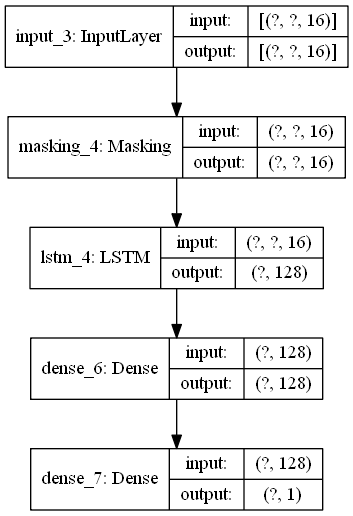
\includegraphics[scale=0.4]{Small Model with dense.png}
\label{LSTM Model Diagram with Hidden Dense Layer}
\end{figure}
The chosen hyper-parameters are 128 for the LSTM vector output size and an Adam optimizer with a learning rate of 0.0005 and an epsilon of 1e-8. Models are trained for 70 epochs.

The stochastic nature of the Adam optimizer causes the training of the model to be unstable. However, this problem is especially prevalent when training LSTMs, as has been reported in \cite{StableReccurantModels, LSTMInstability}. This instability problem exacerbates the difficulty of doing a hyper-parameter search. Now, each hyper-parameter combination must be trained and evaluated many times over, which takes a prohibitive amount of time. For this reason, manual hyper-parameter tuning was done.

This instability problem is observed in this project. A total of 102 models, each with the same hyper-parameters and data were trained and evaluated on the same test set. The test and train set accuracy are reported in the below box and whisker plot. The figure also shows the same statistics when overfit models are not included (models with a training accuracy 2\% greater than the test accuracy are deemed to be overfit, leaving a total of 37 models).

\begin{figure}[H]
\centering\caption{LSTM instability}
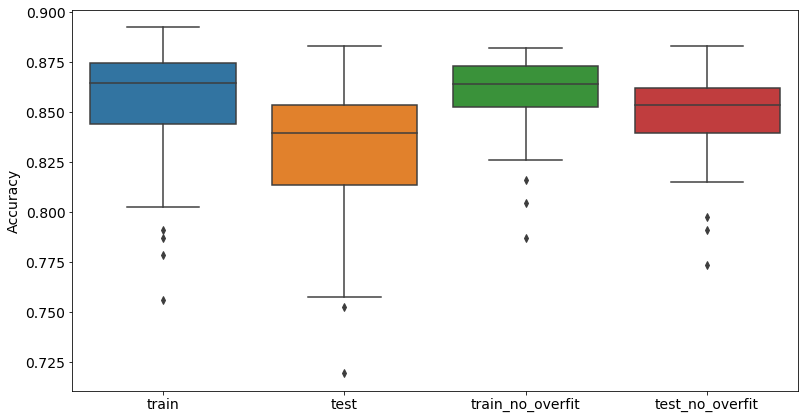
\includegraphics[scale=0.4]{LSTM instability.png}
\end{figure}
% It is hypothesised that in this case, the problem is caused by differences in sequence lengths in batches during training. TODO

The architecture without the extra hidden dense layer was also evaluated. The architecture is the same as in Figure \ref{LSTM Model Diagram with Hidden Dense Layer} but without the dense\_6 layer. 

This model proved to be much more stable. In 129 iterations, only one model had a training accuracy 2\% greater than the test accuracy. The mean test accuracy is \%85 with a standard deviation of 1.6\%. This is compared to the previous model, with a mean test accuracy of 83\% and a standard deviation of 3\%. However, the models training accuracy was slightly decreased, from 85.6\% to 85\%. The below figure shows the box and whisker plot for all 129 models.

\begin{figure}[H]
\centering\caption{LSTM instability no hidden}
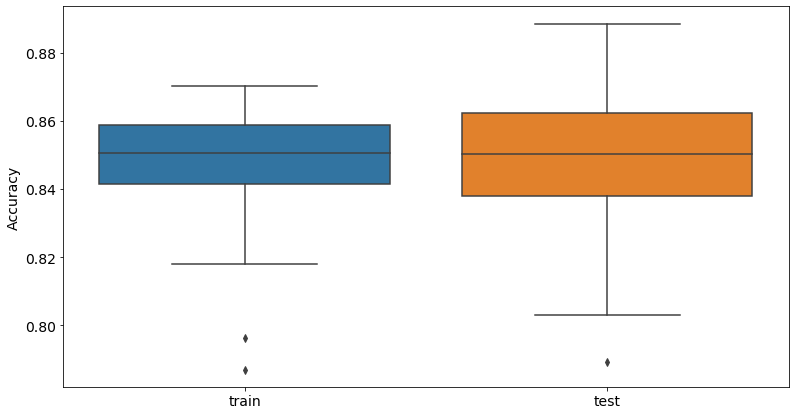
\includegraphics[scale=0.4]{LSTM instability no hidden.png}
\end{figure}
Due to the significantly decreased chance of overfitting and greatly decreased variance, the model with no hidden dense layer will be used for future experiments. 

Next, a single model must be chosen which will be used for future experiments. The next trained model better than 70\% of the previous 129 models was chosen. This model has a test accuracy of 86.8\% and an AUC of 91\%. It has an f1 score for death of 0.75 and for discharge 0.91. This difference between f1 scores is due to the class imbalance. The model can achieve a higher accuracy in the discharge class due to a larger amount of data. Note that class weights have been used during training. 

% This difference between accuracy scores could be due to a difference between the test and train set, such as a difference in average sequence length (TODO).

The below figure shows how accuracy is affected by increasing the sequence length of the test set from admission. This is comparable to Figure \ref{Random Forest Admission} except that in this case, the model is not retrained at every different length. 
The model is trained to, given a complete time series, predict if the patient died. Therefore, the model can only be expected to perform well on complete sequences. The percentage of complete sequences is the green line. Out of these complete sequences, the percentage of patients discharged is shown in orange. As the days of admission data increases, this converges to the baseline accuracy for always guessing discharged. Note that this does not represent the baseline accuracy, as incomplete sequences are also evaluated. 
\begin{figure}[H]
\centering\caption{LSTM Admission Data}
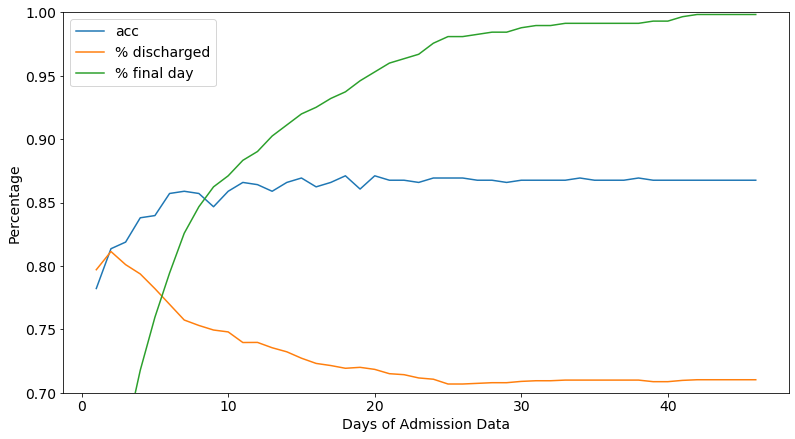
\includegraphics[scale=0.4]{LSTM Admission Data.png}
\end{figure}

The below figure shows the effect of increasing the sequence length of the data, but from the end of the sequence instead of the start (as in the above figure).

\begin{figure}[H]
\centering\caption{LSTM Accuracy Using Number of Days from Discharge or Death}
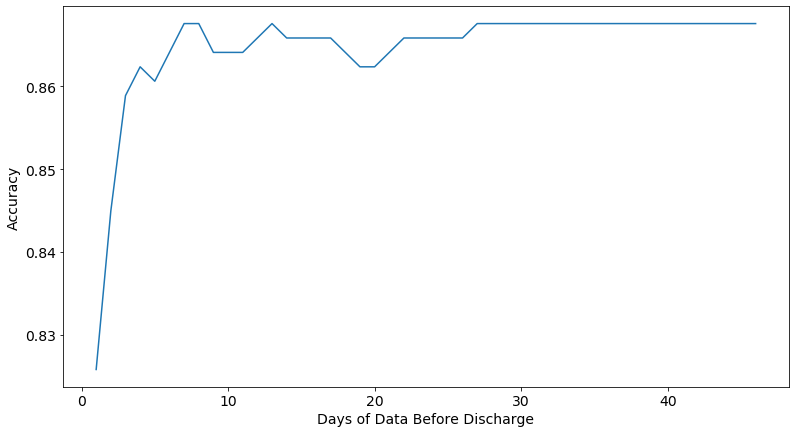
\includegraphics[scale=0.4]{LSTM Accuracy Using Number of Days from Discharge or Death.png}
\label{LSTM Accuracy Using Number of Days from Discharge or Death}
\end{figure}
%TODO future work, compare overfit or less accurate explanations?

Code for this experiment can be found in the `MIMIC death' notebook. 

\subsection{Discussion}

The LSTM has an accuracy of 87\% compared to the random forests accuracy of 84\%. This is a significant increase for machine learning, and was expected since the LSTM has access to more data and therefore should have more predictive power. However, the f1 scores for death are very similar. The LSTM had an f1 score of 0.75 for the death class and 0.91 for the discharge class, while the RF had an f1 score of 0.74 for death and 0.89 for discharge.

These models have lower f1 scores for death compared to discharge, showing that they are better at classifying discharge than death. This is despite employing class weights for both models. One paper uses oversampling of the minority class (death) to overcome this imbalance \cite{ICUFancyLSTM}. However, it is shown in \cite{ImbalancedData} that oversampling can come at the cost of overall accuracy. Future work would be to investigate the effect of oversampling on the models. 

The admission random forest has an AUC of 0.815. This is in line with the findings of the following literature review, which found that machine learning studies with 1000 to 10000 patients had a median AUC of 0.82 for predicting mortality (n=47) \cite{MLICUSystematicReview}. 

When trained on only data from the day of discharge or death, the random forest achieves an accuracy of 84\% (See Figure \ref{Random Forest Discharge}). The LSTM has a smaller accuracy of 82.5\% when evaluated on the same test set, using only the final day data. This difference is quite significant, and it shows that the random forests are a better choice for simply doing classification using 2D data.

We can also conclude that the LSTM model is using more than the final day data from Figure \ref{LSTM Accuracy Using Number of Days from Discharge or Death}. The accuracy greatly increases from 82.5\% to when there's only final day data to 86\% when there's 5 complete days of data, and again to 86.8\% for 7 complete days. The model was trained to predict if the patient died after the final day of data, and adding more data before the final day increases accuracy.

In Figures \ref{Random Forest Admission} and \ref{Random Forest Discharge}, increasing the number of days of data decreases both test and train accuracy (for at least the first 8 days, where there is sufficient data). This could be due to the smaller amount of data available as the number of days increased, as shown in Figure \ref{Random Forest Admission Data}. While the overall accuracy decreases, the f1 score for the test set increases. This is due to the classes becoming balanced, which occurs when the discharged and death lines (red and green) approach 0.5. 

Figure \ref{Random Forest Admission Data} shows another advantage of using time series models. Since these models are able to use any amount of data, there is more data available for training. This is in comparison with some models that can only take a fixed amount of data. For example, a model trained on 1 week of ICU data is useless to a patient only in ICU for 5 days. Also, since time series models are able to use more data for training, they are more likely to be good models in general. 

\section{Explainability}
In this section, the SHAP explainability method is investigated. 

\subsection{SHAP}

SHAP was previously introduced in Section 4.4. 

There are three properties that SHAP is shown to show in \cite{SHAP}. The first is local accuracy, which states that the explanations for all features add up to the actual output from the model. The second is missingness, which states that `missing' features have no impact. The third is consistency, which states that if a model changes so that some input's contribution increases or stays the same regardless of the other inputs, that input’s attribution should not decrease. 

There are different versions of SHAP made for different purposes. The SHAP versions of interest in this paper are TreeExplainer and Kernel SHAP. Both of these methods require a model, which is any python function for Kernel SHAP and an XGBoost model for TreeExplainer. SHAP also always requires a dataset which are the points that will be explained. In the following sections, the test set is used for this.

Kernel SHAP is a the model agnostic version of SHAP. In order to use Kernel SHAP, a background dataset is required. This is used to simulate a `missing' feature by replacing the value with those in the background dataset, which lets SHAP observe the change in the model and calculate the features importance (From the SHAP documentation for KernelExplainer \cite{SHAP}).

TreeExplainer was first introduced in \cite{SHAPInteraction} and detailed further in \cite{TreeExplainer}. It is an optimized version of SHAP made for random forests, and works with random forests created with XGBoost. It is of special interest due to the ability to calculate interaction values, which quantify how features interact with other features. This approach also doesn't require a background dataset, instead it creates a background distribution from following the individual trees and finding how many samples visit each leaf (From the documentation on TreeExplainer \cite{SHAP}).

Firstly, Kernel SHAP is used on the time series data. A modified version of Kernel SHAP is created to better suit time series data and is investigated. Finally, TreeExplainer is used to explain the predictions from the random forests from the previous section. 

\subsubsection{Time Series SHAP}
\label{Time Series SHAP}
As mentioned in Section \ref{SHAP Intro}, there is no support for time series data in SHAP. The 3D data must therefore be turned into 2D data. In this section, Kernel SHAP is used. Kernel SHAP uses a model, which is a user supplied python function. This function should take the a 2D input (array of inputs) and return a 1D array with the model outputs for each input. This is different to the input and output of the LSTM model. The input is reshaped to (num\_input\_days, 1, num\_features), meaning the model treats each of the inputs as a different time series with length 1. The output from the LSTM is flattened to a 1D array. 

SHAP also requires a background dataset. Using the entire test set as a background dataset would take a prohibitive amount of time. Instead of this, a summary dataset of 10 points is chosen using the k-means function. Finally, the SHAP values are calculated from the test dataset, where the data is made to be 2D by removing the sequence IDs. 

SHAP is now run for every data point, which takes approximately 37 minutes. The output from this is a SHAP value for every feature for every day. An example of some SHAP values from a single day is visualized in the force plot below. In this day, a heart rate with a value of 120 pushes the prediction towards mortality, while the platelet count, HCO3, haemoglobin and age all push the prediction towards survival. The SHAP values are the length of the bar for the feature, where the red bars have a positive value and the blue bars have a negative value. These values sum up to the actual prediction from the model for this day.

\begin{figure}[H]
\centering\caption{SHAP Explanation Example}
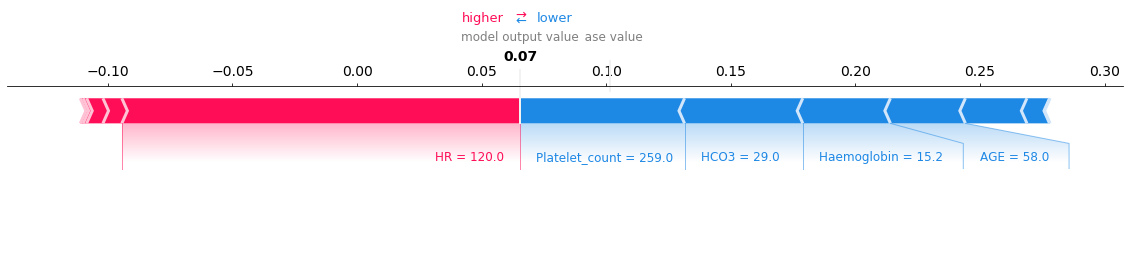
\includegraphics[scale=0.35]{SHAP individual explanation.png}
\end{figure}

The below figure shows the global explanations. These are formed by taking every SHAP value for every feature, plotting the value and shading the point by the feature value. This can help create global explanations such as that decreasing HCO3 increases likelihood of mortality, older patients are at a greater risk and a higher heart rate is associated with a higher mortality rate. However, there appears to be a more complex relationship for platelet count, where low values increase the likelihood of mortality but so do very high values.

\begin{figure}[H]
\centering\caption{Vanilla SHAP Global Explanations}
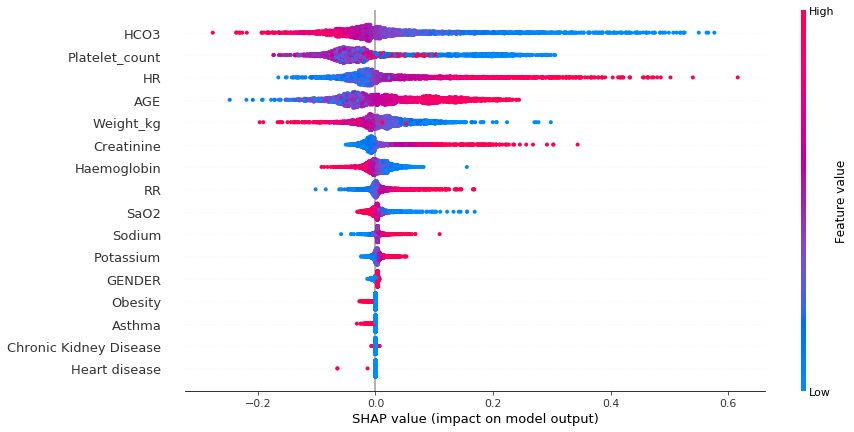
\includegraphics[scale=0.4]{Vanilla SHAP Global.png}
\label{Vanilla SHAP Global}
\end{figure}

The above plot also sorts features by importance. This can help provide more global insight, such as that HCO3 is the most important feature that the model is using to make their prediction, and the comorbidities (the bottom 4 features) seem to have little effect, and when they do they bring the model towards survival. 
The importance is quantified by calculating the mean absolute SHAP value, as can be seen in the below figure. This allows conclusions such as HCO3 is twice as important as weight in general. 

\begin{figure}[H]
\centering\caption{SHAP Feature Importance }
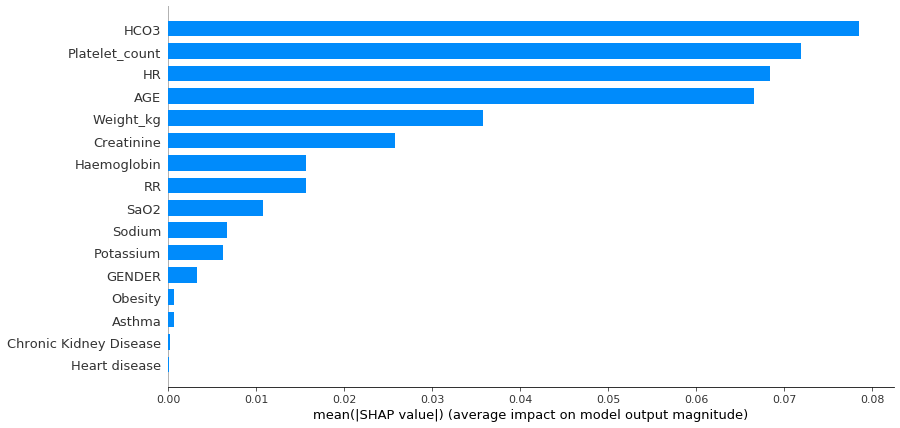
\includegraphics[scale=0.4]{Vanilla SHAP Feature Importance.png}
\end{figure}

\cite{ICUFancyLSTM} also uses vanilla SHAP to create global explanations. They find similar trends for age, heart rate, creatinine and platelets. However, the importance of these features are different to the results obtained in this study. Age is the most important feature (i.e. appears on top in the global explanation figure), followed by heart frequency, creatinine and platelets.

This paper also finds that comorbidities have a lesser effect than the majority of bio-marker features, and some result in a lower mortality rate. This paper concludes that this is likely due to the model being unable to learn meaningful relationships due to the small number of patients with comorbidities.

SHAP can be used to show more interesting global relationships. The below figure shows plots for the top 4 most important features for this model (see Figure \ref{Vanilla SHAP Global}), as previously seen in Figure \ref{SHAP Example Systolic BP}. Note that the axis are different for each subplot. Similar plots for all other features can be found in (Appendix A).

\begin{figure}[H]
     \centering
     \begin{subfigure}[b]{0.47\textwidth}
         \centering
         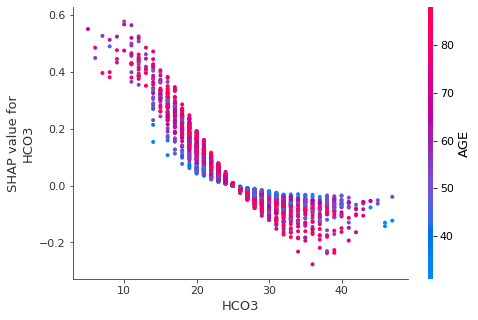
\includegraphics[width=\linewidth]{Vanilla SHAP Global/Vanilla SHAP Global for HCO3.png}
         \caption{HCO3}
     \end{subfigure}
     \hfill
     \begin{subfigure}[b]{0.47\textwidth}
         \centering
         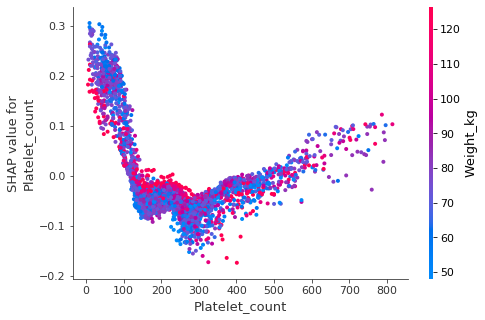
\includegraphics[width=\linewidth]{Vanilla SHAP Global/Vanilla SHAP Global for Platelet_count.png}
         \caption{Platelet Count}
     \end{subfigure}
     \hfill
     \begin{subfigure}[b]{0.47\textwidth}
         \centering
         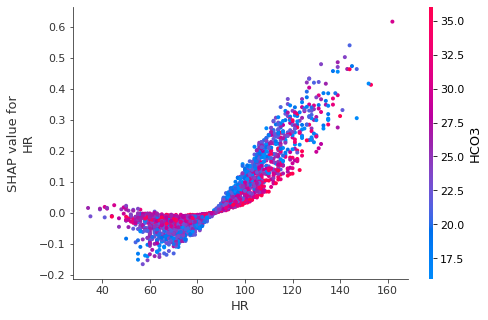
\includegraphics[width=\linewidth]{Vanilla SHAP Global/Vanilla SHAP Global for HR.png}
         \caption{Heart Rate}
     \end{subfigure}
     \hfill
     \begin{subfigure}[b]{0.47\textwidth}
         \centering
         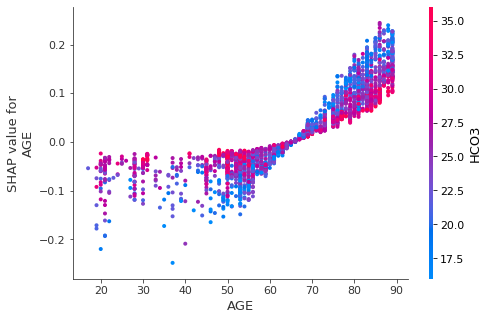
\includegraphics[width=\linewidth]{Vanilla SHAP Global/Vanilla SHAP Global for AGE.png}
         \caption{Age}
     \end{subfigure}
     \caption{SHAP Explanations for Individual Features}
        \label{Vanilla SHAP Global Features}
\end{figure}

The average from the entire dataset for HCO3, platelet count, heart rate and age are 25.5, 233, 86.7 and 65.8. For three of the plots in Figure \ref{Vanilla SHAP Global Features}, all points that are equal to the mean have a SHAP value of 0. A SHAP value of 0 implies the feature has no effect on the prediction. This means the model has learned that having the mean value for any of these features does not help classify the point.

The exception is for platelet count, where the mean value has a range of SHAP values between -0.1 and 0. The model has clearly learned a more complex relationship with this feature than others. Values too low or too high increases mortality. Also, patients with a greater weight have a higher mortality than those with a lower weight only when the platelet count is between 150 and 300. It is proposed that the W shape of this function is caused by the use of k-means to approximate the background samples. While the 10 points of background samples are appropriate for many other features, platelet count has a larger range of 810, a mean of 240 and a standard deviation of 147.

Besides the mean, most other values of features result in a spread of SHAP values. For example, a heart rate of 120 has resulted in a range of SHAP values between 0.1 and 0.5. This is due to the interactions that heart rate has with other features. Each feature in Figure \ref{Vanilla SHAP Global Features} is also plotted with a colour bar representing the strongest interacting feature. We can see that heart rate interacts strongly with HCO3. For example, a heart rate of 120 on a day with high HCO3 results in a lower SHAP value than it does on a day with a low HCO3.

We are able to use SHAP to create rich global explanations. However, local explanations, specifically explanations about a complete time series, are not accurate. This is because each day of data in a sequence is evaluated individually, meaning the actual output from the model is different when compared to the outputs from the SHAP model.

An example of this is featured below. The model predictions are calculated from SHAP by summing up the SHAP values for all features in that day and adding the expected value. The model output line is created by evaluating the time series with all days up to and including the current day, representing the actual prediction by the model. Note that the two match only on the first day.

\begin{figure}[H]
\centering\caption{SHAP Local Explanation Example}
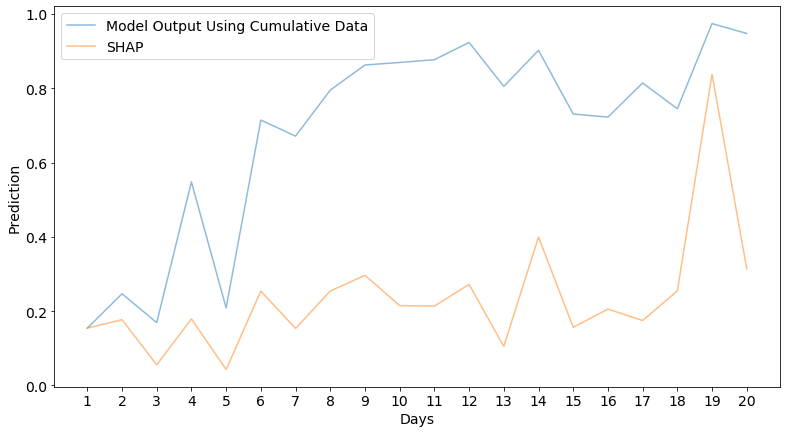
\includegraphics[scale=0.4]{Vanilla SHAP local1.png}
\label{SHAP Local Explanation Example}
\end{figure}

The below shows the same trend as the above but for the first 20 sequences in the test set instead of just one. Note that the sequence ID goes back to 0 for readability. This also shows a general trend where the actual model always has a prediction greater than that of using just one day of data. This could suggest that the model has learnt that a longer stay in ICU increases risk of dying.

\begin{figure}[H]
\centering\caption{SHAP Local Explanation Examples}
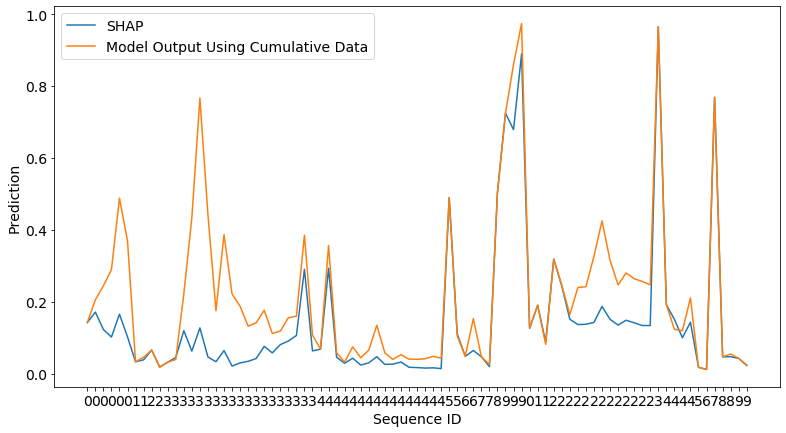
\includegraphics[scale=0.4]{Vanilla SHAP local2.png}
\label{SHAP Local Explanation Examples}
\end{figure}

This shows that the local accuracy property of SHAP is broken, and therefore that the local explanations do not match the model.

\subsubsection{Time Series SHAP Modifications}

By exploiting the nature of LSTMs and their hidden state, SHAP can be modified to better handle time series data. The idea of using the hidden state of the LSTM in SHAP is inspired by \cite{TimeSeriesSHAP}, however the implementation and ML framework used in this section is entirely new. Again, Kernel SHAP is used.

The general strategy is to store the hidden state from the LSTM and use it for the next element in the sequence in the time series. This way, the model will have the exact same inputs as when it is being used on time series data. The data is still passed to SHAP as in the above section (i.e. 2D data).

Firstly, modifications to the model had to be made. It must be able to take the internal states as inputs, therefore two new InputLayers are required. Also, it must return these states as outputs, resulting in two extra outputs. The new model architecture is shown in the below figure.

\begin{figure}[H]
\centering\caption{Updated LSTM Model}
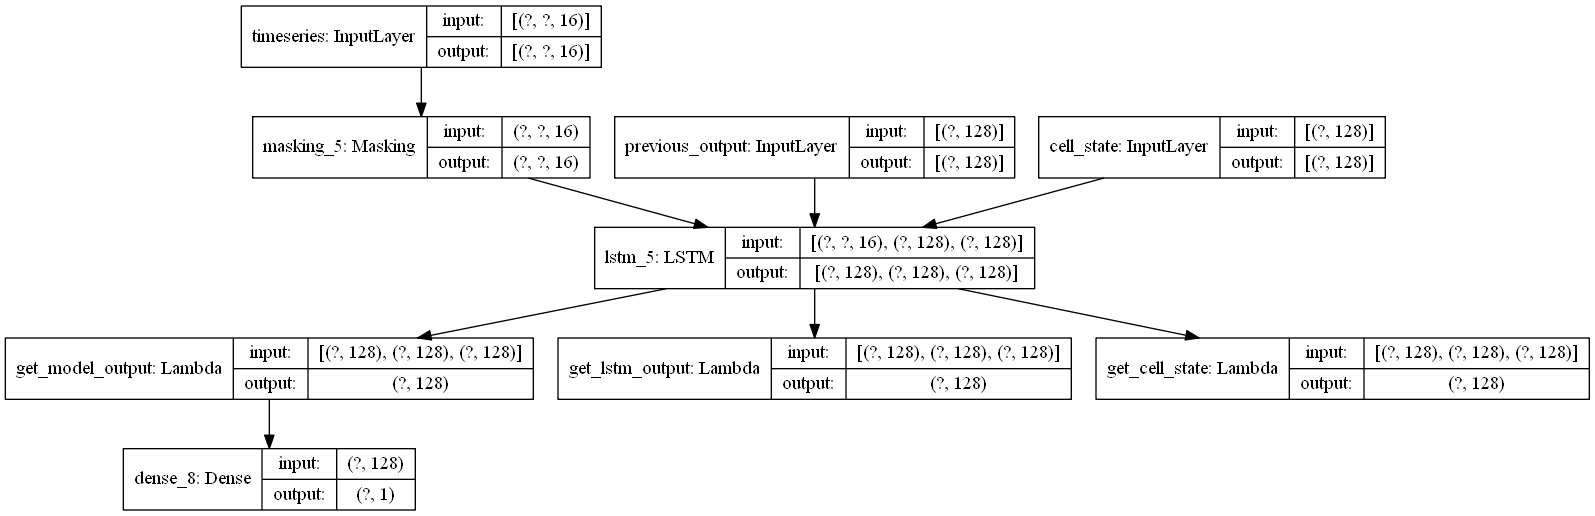
\includegraphics[scale=0.25]{BIG model.png}
\end{figure}
Note that the model is still able to take arbitrary length sequences. The hidden state is only used at the first element in the sequence, and the hidden state is only returned from the last element. There are now two ways to run the model on time series data: Inputting the entire time series of length N with an empty initial state. Running the model N times, once with each day of data, using an empty initial state for the first day, and on subsequent days using the returned hidden state from the previous day.

The SHAP function `shap\_values' was extended to take an extra argument, `association', as well as the existing X argument for the dataset. `association' is an array where the $i$th element is the ID of the sequence that the $i$th piece of data in X belongs to. For example, if the first two time points in the dataset X correspond to the same time series, the association array could be [1,1], or anything as long as the first two values in are equal. In this dataset, the `HADM\_ID' from each element is used as the association array.

SHAP is modified to save the LSTM output and cell state for each time. This saved state is fed into the model the next time data that has the same sequence ID is evaluated. 

SHAP is able to pass in and get hidden state from the LSTM through a simple API. The `model' function that is given to SHAP must now take an optional argument `internal\_state'. If None, this will evaluate the input with default initialization. Otherwise, this function should expect a list of the form [h, c] where h is the previous LSTM output and c is the previous cell state. This input should be given to the underlying LSTM. Finally, this `model' function should return a list of the form [output, h, c], where output is the model output, h is the LSTM output and c is the new cell state. This means a wrapper function is needed to run the model. 

These SHAP changes are backwards compatible, and the above API is only used when an `association' array is given. 

The above API works for LSTM models or other models which take 3 inputs and give 2 outputs. Very minor modifications would be required to run the equivalent model on other time series models that take a different number of arguments, e.g. gated recurrent units (GRUs).

This API of using an association matrix is chosen to simplify the implementation. The alternative is to modify SHAP further to take an array and run all the elements in SHAP in a single call, as in \cite{TimeSeriesSHAP}. However, this adds unnecessarily complexity to the implementation. If this API is desired, it can be created using the association array method by making the library create an association matrix automatically if a 3D data set is provided. 

Details on code modifications to the SHAP library and a link to the repository can be found in Appendix B. Functionality required to run this new SHAP can be found in the `MIMIC death' notebook under the `New SHAP LSTM Design' section. 

\subsubsection{Time Series SHAP Evaluation and Sanity Checks}

SHAP has three desirable theoretical properties. The properties are as follows.

\textbf{Property 1 - Local accuracy}

The SHAP paper describes this property as follows. ``When approximating the original model for a specific input, local accuracy requires the explanation model to at least match the output for the simplified input'' \cite{SHAP}. In other words, the sum of all SHAP values in an explanation should be the same as what the model actually output. This property is clearly desirable, since if it was not satisfied the predictions might not be relevant to the actual model. 

This property is held in the modified SHAP on the scale of entire time series. If one assumes that the property holds in the original SHAP, since the modified SHAP is running exactly the same model as the actual LSTM the property will hold for the modified SHAP. This can be verified in practice by checking that the sum of all SHAP values from the final time step in a sequence is the same as the output from the model when using the entire sequence.

This validation is done for the ICU dataset. 

\textbf{Property 2 - Missingness}

This property is described as follows. ``If the inputs represent feature presence, then missingness requires features missing in the original input to have no impact''\cite{SHAP}. This property is used when calculating the SHAP value. To determine the impact of a feature, that feature is set to "missing" and the change in the model output is observed (From the SHAP documentation for KernelExplainer \cite{SHAP}). In practice, this is simulated by replacing the feature with values from the background dataset. Interestingly, this property is not satisfied in Figure \ref{Vanilla SHAP Global Features} for platelet count, as there is no value that acts as a missing input.

This property cannot be satisfied in general for time series models due to the presence of the hidden state. An example that would be impossible to satisfy is a model that counts the length of a time series. Every data point will increase the prediction by 1, meaning that if there is only 1 feature the SHAP value will be 1 no matter what the input is.

\textbf{Property 3 - Consistency}

This property is described as follows \cite{SHAP}. ``Consistency states that if a model changes so that some simplified input’s contribution increases or stays the same regardless of the other inputs, that input’s attribution should not decrease.'' 

In order to find if the contribution increases or stays the same regardless of the other inputs, this property relies on the missingness property. This means that this property also cannot satisfied in general.

\textbf{Addition LSTM}

The new SHAP is evaluated using a simple addition LSTM model. This addition LSTM is designed to add numbers in a sequence and return the result. The model has two features, the first is a random integer between 0 and 10, and another feature that is always 1. 
The extra feature is added both to test SHAPs behaviour and also to differentiate between an empty feature and a value of 0. The LSTM is trained to add all of these numbers together. 

The training set is created with sequences of a random length between 1 and 10. The training and test sets both are created with 1000 sequences. The same LSTM as in Section \ref{LSTM} is used, however the loss is now mean squared error since this is a regression problem. The model attains a mean squared error of 0.7 on the train set and 0.3 on the test set.

The below figure shows the global explanations from vanilla SHAP for this LSTM. Note that this SHAP value is relative to the expected value from the model that SHAP estimates, which in this case is 3.1. We can see the inputs for Feature 0 are evenly grouped from -2 to 7. 
Since all these groups have the same colour (i.e. feature value), it is clear that the same integer results in exactly the same SHAP value. Remembering that the model is adding 1 at each time step, this comes to a range from 0 to 9, which is the same as the input values for this feature. Furthermore, Feature 1 always has a SHAP value of 0. This suggests that the model has learned to ignore this feature.

\begin{figure}[H]
\centering\caption{Addition LSTM Global Explanations}
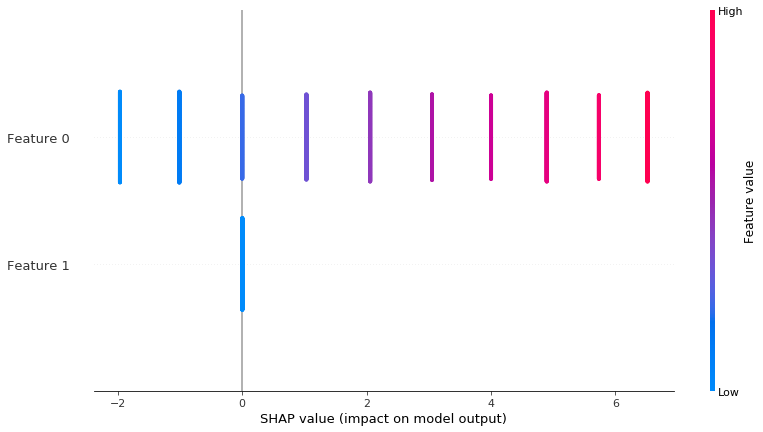
\includegraphics[scale=0.4]{Sanity Old Global.png}
\end{figure}
This is also shown in the below figure. 

\begin{figure}[H]
\centering\caption{Addition LSTM Global Explanation for Feature 0}
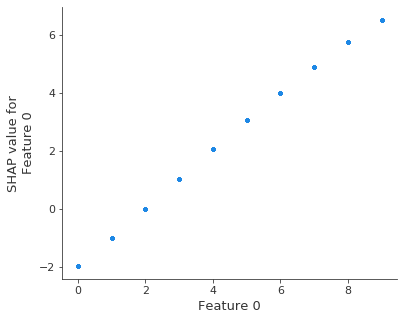
\includegraphics[scale=0.5]{Sanity Old Global Feature.png}
\end{figure}
As before, the local explanations do not match the actual models output. This can be seen in the figure below, which shows the SHAP values (y axis) for the different element ID (x axis). The LSTM is adding the sequence (7,0,7,1,8,1,2,3,7). Note that the feature switches from red to blue depending on which side of the expected value the result is, and feature 1 has no effect. 

\begin{figure}[H]
\centering\caption{Addition LSTM Local Explanation}
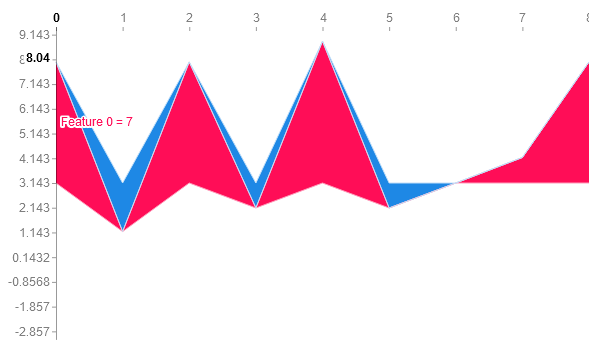
\includegraphics[scale=0.6]{Sanity Old Local.png}
\label{Sanity Old Local}
\end{figure}

The results are very different for the new SHAP. Since the new SHAP adheres to the local accuracy property, the same input will no longer have the same SHAP value. This is because the output will depend on what elements the LSTM has already seen. For example, if the previous sum is 5 and the new SHAP value is 0, the model will output 6 for the new element, which means the features must have a SHAP value of 6.

This behaviour is shown in the below figure. The expected value from SHAP is now 5.5. Clusters of matching SHAP values can still be seen. However, there is now no longer a clear relationship between feature value and SHAP value. Note that Feature 1 still has no importance. 

\begin{figure}[H]
\centering\caption{Addition LSTM New SHAP Global Explanations}
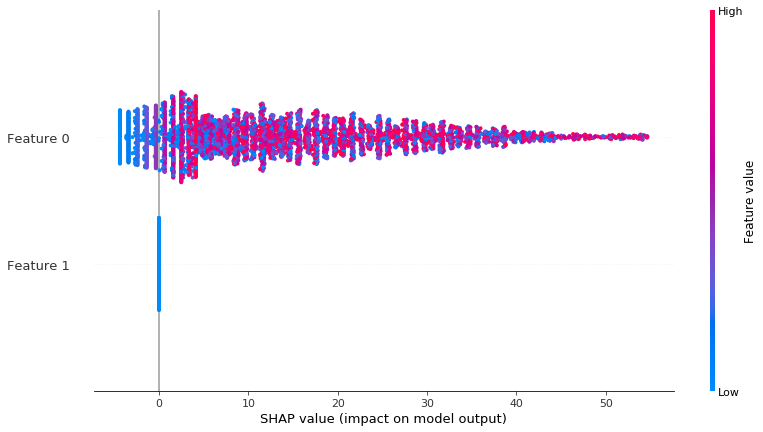
\includegraphics[scale=0.4]{Sanity New Global.png}
\end{figure}
This is shown more clearly in the below figure. When Feature 0 is 0, the SHAP value can be anywhere up to 50. 

\begin{figure}[H]
\centering\caption{Addition LSTM New SHAP Global Explanation for Feature 0}
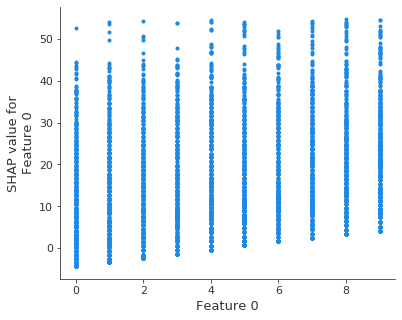
\includegraphics[scale=0.5]{Sanity New Global Feature.png}
\end{figure}
While the global explanations are not functional, the local explanations are correct across an entire time series, as can be seen below. This is the same sequence as in\ref{Sanity Old Local}

\begin{figure}[H]
\centering\caption{Addition LSTM New SHAP Local Explanation}
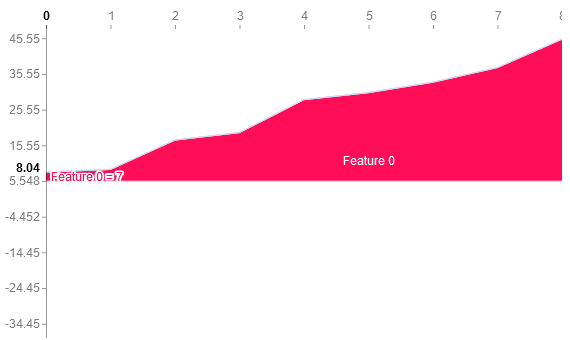
\includegraphics[scale=0.6]{Sanity New Local.png}
\end{figure}

This experiment has shown that the new SHAP gives accurate local explanations at the cost of inaccurate global explanations. One possible modification to attempt to get both accuracy local and global explanations is to try extract the contribution from the hidden state. For example, if the previous sum was 15 and the current sum is 20, then 15 can be extracted for the hidden state, and the current features will make up the remaining 5. 

Unfortunately, this is a simplification that is unlikely to work in general. For example, consider a counter LSTM that counts the number of elements in the sequence. No features should have any importance since the LSTM will increment irrespective of the feature value, however both old and new SHAP will atribute 1 to the features. Also, consider an LSTM that acts as both a counter but also has complex interactions between the hidden state and the current values. There is no way to tell how much of the hidden state is due to the LSTM counting and how much is due to these other interactions.

Code for this experiment is available in the `SHAP Sanity Checks' notebook, see Appendix A.

\textbf{ICU LSTM}

Firstly, it is verified in code that the ICU LSTM satisfies the local accuracy property for all elements in the test set. 

The global explanations for the same model as in Section \ref{Time Series SHAP} is done using the new SHAP. Because the output from the model is between 0 and 1, the global explanations do not suffer from the same problems as the addition LSTM. In fact, the global explanations seem to match those in Figure \ref{Vanilla SHAP Global}, and the features have the same order of importance. 

\begin{figure}[H]
\centering\caption{New SHAP Global Explanations}
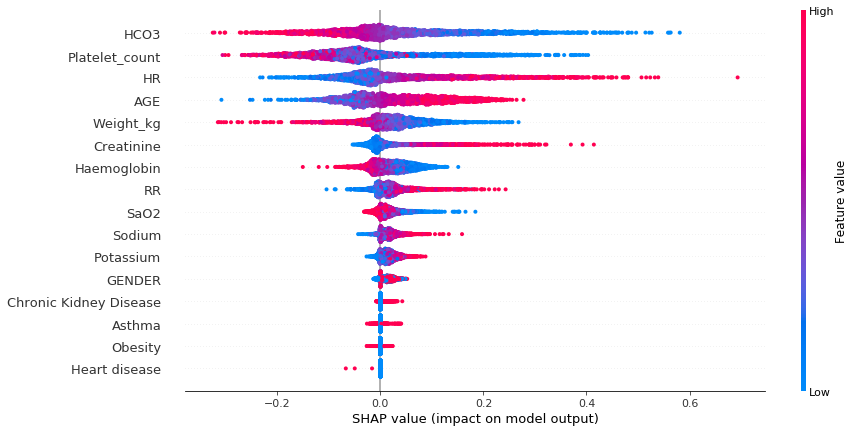
\includegraphics[scale=0.35]{New SHAP Global.png}
\end{figure}

However, the below individual plots for features show the problems that the new SHAP has. Specifically, the mean value for HCO3, heart rate and age no longer have 0 SHAP value. The most important interactions are also different.

\begin{figure}[H]
     \centering
     \begin{subfigure}[b]{0.47\textwidth}
         \centering
         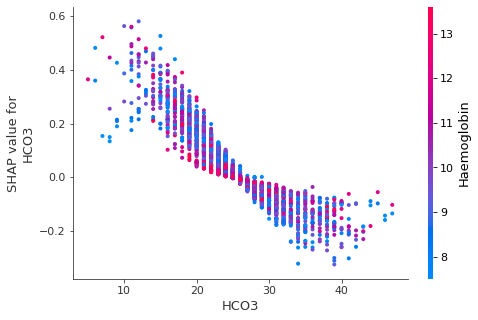
\includegraphics[width=\linewidth]{New SHAP Global/New SHAP Global forHCO3.png}
         \caption{HCO3}
     \end{subfigure}
     \hfill
     \begin{subfigure}[b]{0.47\textwidth}
         \centering
         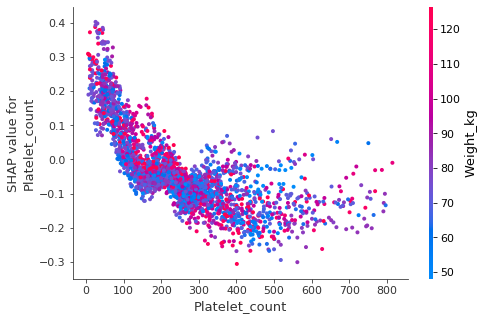
\includegraphics[width=\linewidth]{New SHAP Global/New SHAP Global forPlatelet_count.png}
         \caption{Platelet Count}
     \end{subfigure}
     \hfill
     \begin{subfigure}[b]{0.47\textwidth}
         \centering
         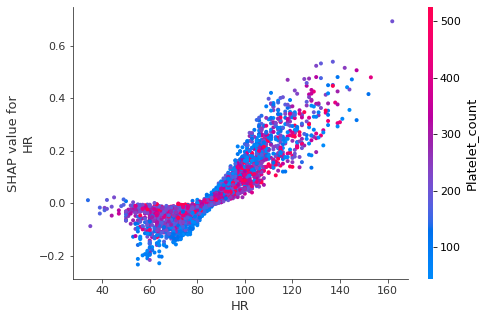
\includegraphics[width=\linewidth]{New SHAP Global/New SHAP Global forHR.png}
         \caption{Heart Rate}
     \end{subfigure}
     \hfill
     \begin{subfigure}[b]{0.47\textwidth}
         \centering
         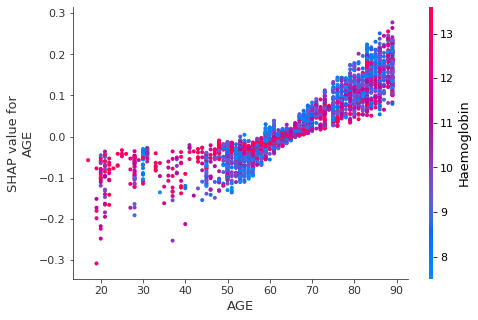
\includegraphics[width=\linewidth]{New SHAP Global/New SHAP Global forAGE.png}
         \caption{Age}
     \end{subfigure}
     \caption{New SHAP Explanations for Individual Features}
\end{figure}

A local explanation over an entire time series is shown below for vanilla and new SHAP. The same 19 day ICU stay is explained. Note that the actual model output is where the blue and red lines meet (each red line represents a feature that impacts towards mortality, and blue lines impact towards survival). This shows how inaccurate the LSTM is when only evaluated on single day slices. According to Vanilla SHAP, the patient will be discharged alive but the actual model is very confident the patient will die, even after the first week of ICU data.

\begin{figure}[H]
     \centering
     \begin{subfigure}[b]{0.47\textwidth}
         \centering
         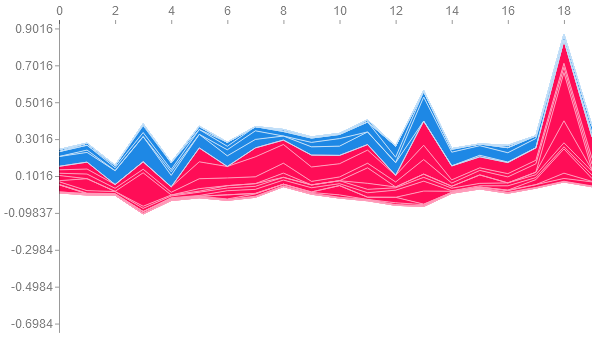
\includegraphics[width=\linewidth]{Vanilla SHAP Local ICU.png}
         \caption{Vanilla SHAP}
     \end{subfigure}
     \hfill
     \begin{subfigure}[b]{0.47\textwidth}
         \centering
         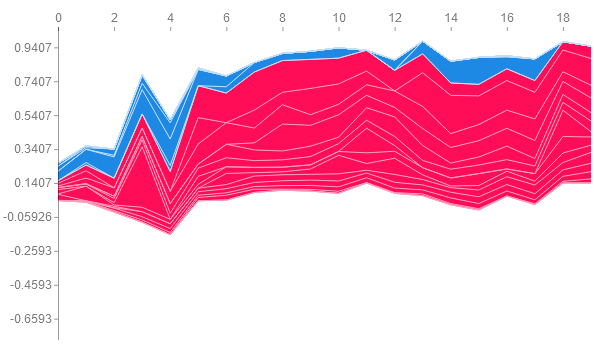
\includegraphics[width=\linewidth]{New SHAP Local.png}
         \caption{New SHAP}
     \end{subfigure}
     \caption{SHAP Local Explanations}
 \label{SHAP Local Explanations}
\end{figure}

This also highlights an interesting relationship, that longer series have a higher chance of mortality. The mean prediction over all days of data is 0.25 for vanilla SHAP, but it is 0.37 for the new SHAP. For 1969 out of 2787 days of the data, the SHAP values from new SHAP are larger than those from vanilla SHAP. This could suggest that the LSTM has learned that the longer the stay in ICU, the higher the chance of mortality. In order to test this, the `day' feature could be added as an input to the model. 

The vanilla SHAP plot in Figure \ref{SHAP Local Explanations} shows some moderate jumps in mortality (spikes), such as in day 3 and 13 and also a large spike at day 18. In this specific example, the spikes at day 3 and 19 are caused by a very high heart rate. This shows another use for vanilla SHAP. It can be used to detect such spikes which may go unnoticed by the new SHAP due to a consistently high mortality prediction. Future work would be to investigate this possibility. 

% Alina's question: did the model learn to differentiate when bad things happen in 1 day or slowly? just use old SHAP to look for `spikes'. 

\subsubsection{TreeExplainer}

In this section, TreeExplainer is used on the random forest trained on admission data, final day data and the final 2 days of data. In all of these experiments, SHAP runs in less than 1 second.

\textbf{Admission Data}

The first experiment is running the admission random forest that uses only first day data from Figure \ref{Random Forest Admission} with TreeExplainer. The results of the global explanations are in the figure below.

\begin{figure}[H]
\centering\caption{TreeExplainer Global Explanations Admission}
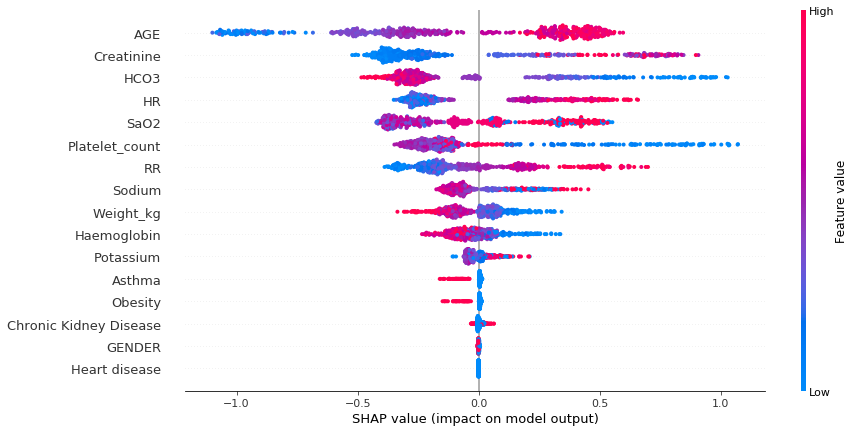
\includegraphics[scale=0.4]{TreeExplainer Admission1 Global.png}
\end{figure}
The features that are deemed important are different to the LSTM from the previous section. Age now has the highest impact on the model. It makes sense why the model would find age more relevant to death since the age is constant throughout the ICU stay, but the biomarker features are likely to be very different from day 1 to the final day. The importance of all features are shown below. Interestingly, weight has a lesser effect than that of the LSTM. This could be due to the lack of interactions formed between weight and other features.

\begin{figure}[H]
\centering\caption{TreeExplainer Feature Importance Admission}
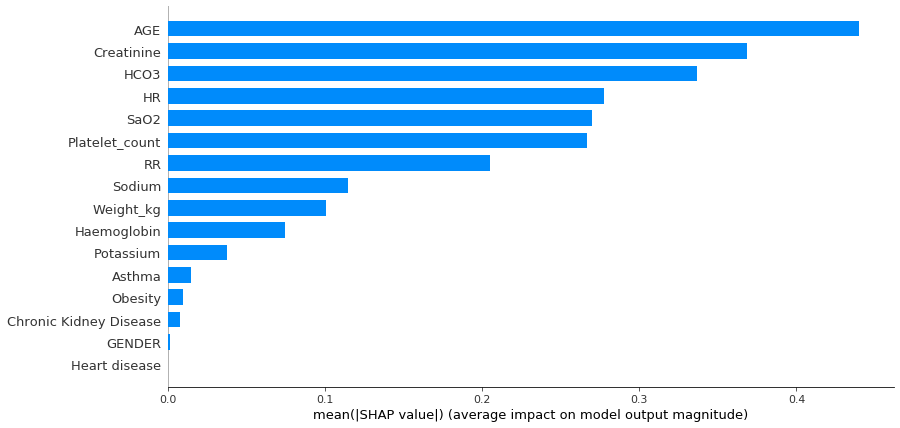
\includegraphics[scale=0.4]{TreeExplainer Admission1 Feature Importance.png}
\end{figure}
% It is possible that the model is only accurate for short time series (i.e. 1 day time series). 
The top 4 features are shown below. Similar trends are noticed for heart rate, age and HCO3 when compared to Figure \ref{Vanilla SHAP Global Features}. However, the lines are less smooth and are not as continuous as they were before. This could be due to the nature of the decision boundaries of random forests, which can be very sharp. However, it is likely due to the model being trained with insufficient data, as the XGBoost survival model featured in \cite{SHAPInteraction} does not have this discontinuity problem. There are also significantly less data points in the test set for this problem, only 574 compared to the LSTM's 2787. 

\begin{figure}[H]
     \centering
     \begin{subfigure}[b]{0.47\textwidth}
         \centering
         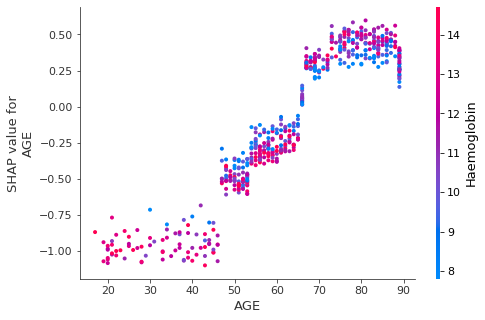
\includegraphics[width=\linewidth]{TreeExplainer Admission1 Global/TreeExplainer Admission1 Global for AGE.png}
         \caption{Age}
     \end{subfigure}
     \hfill
     \begin{subfigure}[b]{0.47\textwidth}
         \centering
         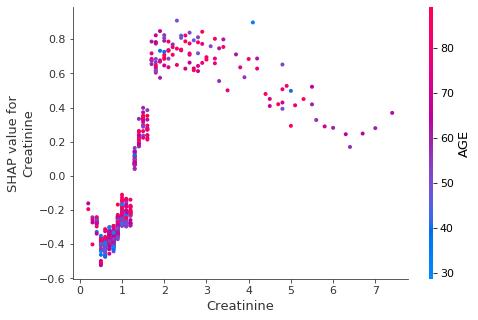
\includegraphics[width=\linewidth]{TreeExplainer Admission1 Global/TreeExplainer Admission1 Global for Creatinine.png}
         \caption{Creatinine}
     \end{subfigure}
     \hfill
     \begin{subfigure}[b]{0.47\textwidth}
         \centering
         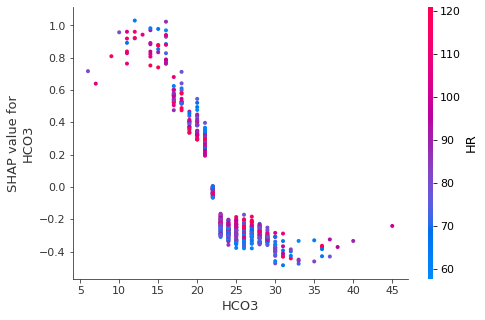
\includegraphics[width=\linewidth]{TreeExplainer Admission1 Global/TreeExplainer Admission1 Global for HCO3.png}
         \caption{HCO3}
     \end{subfigure}
     \hfill
     \begin{subfigure}[b]{0.47\textwidth}
         \centering
         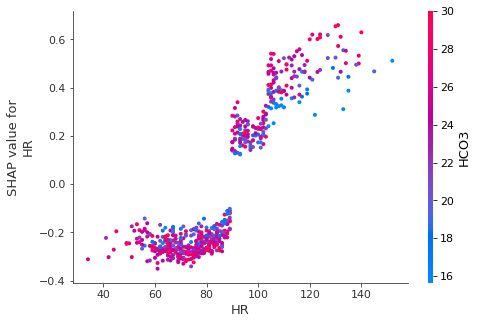
\includegraphics[width=\linewidth]{TreeExplainer Admission1 Global/TreeExplainer Admission1 Global for HR.png}
         \caption{Heart Rate}
     \end{subfigure}
     \caption{SHAP Explanations for Individual Features}
%         \label{Vanilla SHAP Global Features}
\end{figure}

\textbf{Final Day Data}

This experiment is more directly comparable with the LSTM, as it is predicting if the patient died after these readings. This random forest also had a much higher accuracy than the admission random forest by 6\%. 


\begin{figure}[H]
\centering\caption{TreeExplainer Global Explanations Final Day}
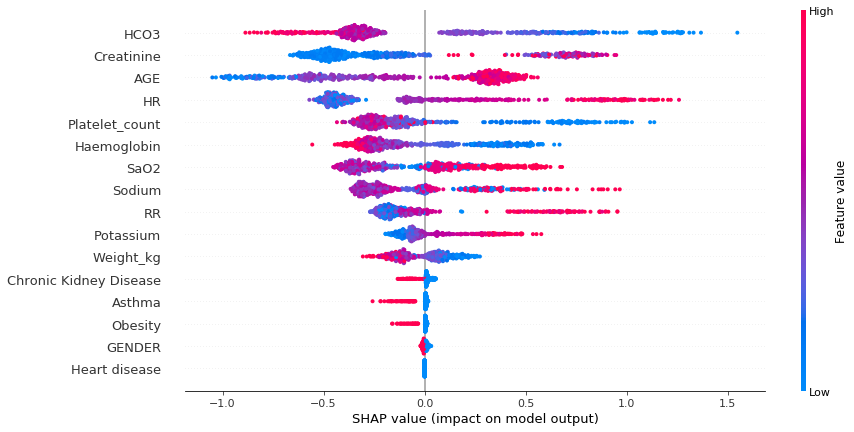
\includegraphics[scale=0.4]{TreeExplainer Final1 Global/TreeExplainer Final1 Global.png}
\end{figure}
The trends (the general shape of the curves) for HCO3, platelet count, age, and heart rate are similar to Figure \ref{Vanilla SHAP Global Features}. However, the trends for creatinine and SaO2 are different. The SHAP values for creatinine in particular have a much larger range. SaO2 has the opposite trend, where a higher SaO2 increases mortality.

The feature importance also differs from the LSTM. Creatinine is one of the most important features for the random forest, similarly to the admission random forest.

\begin{figure}[H]
\centering\caption{TreeExplainer Feature Importance Final Day}
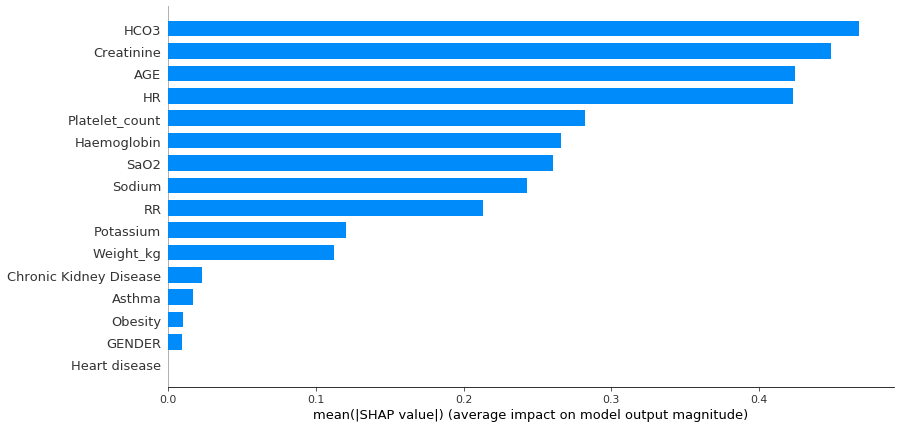
\includegraphics[scale=0.4]{TreeExplainer Final1 Global/TreeExplainer Final1 Feature Importance.png}
\end{figure}
As before, the top 4 features are shown.

\begin{figure}[H]
     \centering
     \begin{subfigure}[b]{0.47\textwidth}
         \centering
         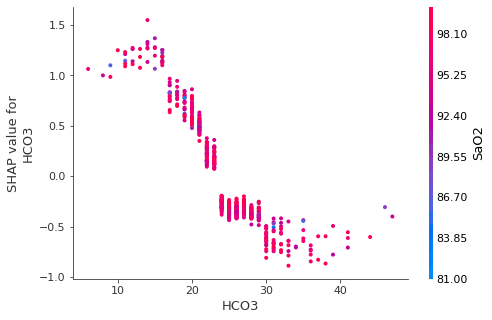
\includegraphics[width=\linewidth]{TreeExplainer Final1 Global/TreeExplainer Final1 Global for HCO3.png}
         \caption{HCO3}
     \end{subfigure}
     \hfill
     \begin{subfigure}[b]{0.47\textwidth}
         \centering
         \includegraphics[width=\linewidth]{TreeExplainer Final1 Global/TreeExplainer Final1 Global for Creatinine.png}
         \caption{Creatinine}
     \end{subfigure}
     \hfill
     \begin{subfigure}[b]{0.47\textwidth}
         \centering
         \includegraphics[width=\linewidth]{TreeExplainer Final1 Global/TreeExplainer Final1 Global for AGE.png}
         \caption{Age}
     \end{subfigure}
     \hfill
     \begin{subfigure}[b]{0.47\textwidth}
         \centering
         \includegraphics[width=\linewidth]{TreeExplainer Final1 Global/TreeExplainer Final1 Global for HR.png}
         \caption{Heart Rate}
     \end{subfigure}
     \caption{SHAP Explanations for Individual Features}
        \label{SHAP Final1 Explanations for Individual Features}
\end{figure}

% Interestingly, heart rate does not have the same relationship with HCO3 as before. It instead interacts mostly with the  

TreeExplainer provides the option to extract interaction values (i.e. the extent that features interact with each other). This makes it possible to see exactly how two features interact, and even plot features without the interactions of other features. 

The figure below shows the main effect of the top 4 features. Since there are no interactions with any other features, there is no longer any variance between the SHAP value for the same value of the feature. When compared with Figure \ref{SHAP Final1 Explanations for Individual Features}, it can be seen that HCO3 and heart rate don't interact much with other features compared to age or creatinine. The discontinuities are clearly evident in these plots.

\begin{figure}[H]
     \centering
     \begin{subfigure}[b]{0.47\textwidth}
         \centering
         \includegraphics[width=\linewidth]{TreeExplainer Final1 Global/TreeExplainer Final1 Main Effect HCO3.png}
         \caption{HCO3}
     \end{subfigure}
     \hfill
     \begin{subfigure}[b]{0.47\textwidth}
         \centering
         \includegraphics[width=\linewidth]{TreeExplainer Final1 Global/TreeExplainer Final1 Main Effect Creatinine.png}
         \caption{Creatinine}
     \end{subfigure}
     \hfill
     \begin{subfigure}[b]{0.47\textwidth}
         \centering
         \includegraphics[width=\linewidth]{TreeExplainer Final1 Global/TreeExplainer Final1 Main Effect AGE.png}
         \caption{Age}
     \end{subfigure}
     \hfill
     \begin{subfigure}[b]{0.47\textwidth}
         \centering
         \includegraphics[width=\linewidth]{TreeExplainer Final1 Global/TreeExplainer Final1 Main Effect HR.png}
         \caption{Heart Rate}
     \end{subfigure}
     \caption{SHAP Main Effect for Individual Features}
%         \label{Vanilla SHAP Global Features}
\end{figure}
An example interaction plot between creatinine and HCO3 is shown below. This plot shows the same interaction as from Figure \ref{SHAP Final1 Explanations for Individual Features}. However, the interaction is now quantifiable. For example, a very high HCO3 is impacts the prediction more when creatinine is between 0 and 1 (0.2 to 0.3) than when it is greater than 1 (-0.1 to -0.2).

\begin{figure}[H]
\centering\caption{TreeExplainer Interaction between Creatinine and HCO3}
\includegraphics[scale=0.5]{TreeExplainer Final1 Global/TreeExplainer Final1 Interaction Creatinine HCO3.png}
\end{figure}

\textbf{Final 2 Days of Data}

In this experiment, the final 2 days of data is used. Day 1 is the data from the second last day of the patients ICU stay, while day 2 is the final day. There are 32 features in total. Global explanations can be seen below. Note that chronic kidney disease, gender, asthma and heart disease for both days are not shown as they have almost no effect.

\begin{figure}[H]
\centering\caption{TreeExplainer Global Explanations Final 2 Days}
\includegraphics[scale=0.4]{TreeExplainer Final2/TreeExplainer Final2 Global.png}
\end{figure}

As expected, the day 2 features have a much greater impact on the model output than those of day 1. The trends for the same feature on different days have the same appearance overall. For example, a low HCO3 increases mortality and a high HCO3 decreases mortality. The quantified feature importance is featured below.

\begin{figure}[H]
\centering\caption{TreeExplainer Feature Importance Final 2 Days}
\includegraphics[scale=0.4]{TreeExplainer Final2/TreeExplainer Final2 Feature Importance.png}
\label{TreeExplainer Feature Importance Final 2 Days}
\end{figure}

The individual feature plots are very similar to those in Figure \ref{SHAP Final1 Explanations for Individual Features}. There are minor differences which could be caused by the difference between the two datasets. 

%TODO add it? ez filler

We can investigate whether or not the model is learning the relationships between the days. One hypothesis for the decrease in accuracy when increasing the days of data is that the random forest cannot learn the relationship between the days. The LSTM is forced to learn this relationship due to it's architecture, but the random forest is not. Interaction between day 2 and day 1 variables. This mimics the way LSTMs work, where features on day 2 interact with previous values, not visa versa.

\begin{figure}[H]
     \centering
     \begin{subfigure}[b]{0.47\textwidth}
         \centering
         \includegraphics[width=\linewidth]{TreeExplainer Final2/TreeExplainer Final2 Interaction HR_day2 day 2.png}
         \caption{HR}
     \end{subfigure}
     \hfill
     \begin{subfigure}[b]{0.47\textwidth}
         \centering
         \includegraphics[width=\linewidth]{TreeExplainer Final2/TreeExplainer Final2 Interaction HCO3_day2 day 2.png}
         \caption{HCO3}
     \end{subfigure}
     \hfill
     \begin{subfigure}[b]{0.47\textwidth}
         \centering
         \includegraphics[width=\linewidth]{TreeExplainer Final2/TreeExplainer Final2 Interaction Creatinine_day2 day 2.png}
         \caption{Creatinine}
     \end{subfigure}
     \hfill
     \begin{subfigure}[b]{0.47\textwidth}
         \centering
         \includegraphics[width=\linewidth]{TreeExplainer Final2/TreeExplainer Final2 Interaction Haemoglobin_day2 day 2.png}
         \caption{Haemoglobin}
     \end{subfigure}
     \caption{SHAP Interaction Effects For Same Feature}
        \label{Vanilla SHAP Global Features final 2}
\end{figure}

There is very little interaction between the features for creatinine and haemoglobin. It appears that HCO3 and heart rate are impacted by the previous day's value. However, the scale on the Y axis shows how little the values are affected. From Figure \ref{TreeExplainer Feature Importance Final 2 Days}, the mean absolute SHAP value for day 2 HR is 0.4, however the day 2 heart rate only changes due to day 1 heart rate by at most 0.04. The relationships shown in the above figure may therefore not be significant.

From the haemoglobin graph in Figure \ref{Vanilla SHAP Global Features final 2}, it is evident that the day 2 haemoglobin goes up to 16 but the day 1 haemoglobin only goes up to 14. The model has learned that if the day 2 haemoglobin is very high it is important to look at the day 1 haemoglobin. 

% This suggests that the model may be looking at trends between the same features. However, since the random forest has so many possible relationships to learn, it does not think of them as important.

Since the random forest is able to handle all features from multiple days at once, there are also interactions between day 1 features and day 2 features (i.e. day 2 features impact on SHAP scores of features from day 1). In fact, the explanations for interaction from day 1 to day 2 look very similar to those in Figure \ref{TreeExplainer Feature Importance Final 2 Days}. If these relationships are significant, the random forest has learned a relationship that does not make sense in the context of the problem.

It is possible that there are many other significant relationships that SHAP interaction plots can show. However, it is unreasonable to interrogate them all. For example, for a 1 week ICU stay with 16 features per day means there will be a total of 112 features, therefore a total of 12544 interactions. Even using 2 days of data has 1024 interactions. This highlights one problem with trying to get detailed explanations for long time series. Even an ideal explainability method that could show the relationship between every feature in the time series so far, it would not be feasible for anyone to check them all. However, if the interactions can be quantified, finding only the most important interactions would be possible.

\subsection{Discussion}

It is found that SHAP is very useful for explaining relationships between features and outputs on a global scale. One of the aims of explainablility is to be able to validate or invalidate a model. SHAP makes this easy to do on a high level, as it can be easily discovered if the model has learned a nonsensical relationship. 

The proposed modifications to SHAP provide local accuracy for entire time series at a cost to the strong theoretical justification of SHAP and global explanations. The Addition LSTM is shown to have meaningless global explanations with the new SHAP but meaningful local explanations. A hybrid use of vanilla SHAP for global explanations and new SHAP for local explanations could be of interest.

It was found that most of the features from the random forests investigated had the same trends. The extra functionality (extracting interactions between features) from TreeExplainer was also investigated, and found to provide rich global explanations. Sensible explanations are also mostly obtained from running a random forest with multiple days of the same features. 

% e.g. compare explanations to medical knowledge, try find weird explanations etc.
% make some conclusions about the model too!

It was found that the explanations from the final day random forest and the LSTM are similar. Future work would involve finding if these relationships are sound in the context of the ICU.

By comparing explanations from the vanilla SHAP to the new SHAP, evidence is found for a relationship between sequence length and mortality. Further investigation is required.

A method that can attribute importance to every feature from all days would be the ideal outcome. This has been shown to be possible for random forests using SHAP, however it is infeasible in it's current state due to an explosion of interactions for long time series. Future work would be to investigate quantifying the most useful interactions to show users. 

This highlights a trade off between greater accuracy and better explanations, since LSTMs are clearly better suited to this problem and attain a significantly higher accuracy.

Another distinction between random forests and LSTMs highlighted in this section is the run time for SHAP. Kernel SHAP takes nearly 40 minutes to run, while TreeExplainer takes less than 1 second for a quarter of the data. This is due to the simplicity of the random forest compared to the LSTM. Note that these run times are on a CPU, however attempts to run the LSTM on a GPU failed. 

\section{Discussion}

The first step in this project was to create a dataset for machine learning. This was done using the MIMIC-III dataset. In order to create the final dataset, a certain subset of features were chosen. These features were chosen due to the number of data points present in the dataset. It was also decided that no imputation would be done in order to simplify the dataset creation.

However, the lack of imputation is a significant limitation. This meant that the study is only using a specific subset of the data, which may have introduced a bias. Clearly there is a larger mortality rate in the final dataset (31\%) compared to the in-hospital mortality rate of all sites in the MIMIC-III study (11.5\%). In future, the MICE method could be used to investigate such biases \cite{MICE}. 

Random forests were created and trained on different amounts of admission or final days of data. Random forests trained on longer time series consistently had a lower accuracy than random forests trained on smaller time series. This is because in the created dataset, the longer the sequence, the less data that is of at least that length. This highlights a further advantage of using time series models, that they are able to use data from every ICU stay, regardless of length.

Two different LSTM models were trained. It was found that a model with an extra hidden layer generalized poorly, while the model without generalized very well. It was also found that the model was not using only the last day of data to make it's prediction. As expected, the LSTM performed better than any of the random forests. 

Three different experiments were done involving SHAP. This includes running SHAP with the LSTM without considering interactions within individual time series sequences. Global explanations are found to be useful and rich. However, it is found that local explanations are incorrect.

A modified version of SHAP is proposed that handles time series data by keeping track of internal state within sequences. Modifications to the SHAP library were created and a new general API was proposed. While these modifications break some ideal properties, it satisfies the local accuracy property on the scale of entire time series. 

An example is shown where this new method does not provide useful global explanations. It is proposed that a hybrid system using vanilla SHAP for global explanations and using the new SHAP for local explanations could be used together.

\section{Conclusion}

This thesis had one key aim; to see if it's possible to predict death using time series ICU data in an interpretable way.

It was shown that an LSTM attains a high accuracy on time series data when predicting death and discharge, however it is better at predicting discharge than death. The accuracy of the model was verified to be higher than that of a model that uses data of a fixed sequence length.

This model was made interpretable by using the SHAP explainability method to create global explanations, and a newly proposed modified version of SHAP to provide local explanations in the scale of individual time series. This allows the model to be interpreted for validation by checking global explanations, ensuring the model aligns with medical knowledge. Local explanations can be used to tell which features are important for a patients current state. 

However, the local explanations do not perfectly describe the model. In particular, it is not able to see precisely how features from previous days affect the current day. This is shown to be possible using SHAP, but only for models that take data of a fixed sequence length. 

While the time series model may have good accuracy and be explainable, is it useful? In practice, models that predict specific times to death or discharge for example would be more useful. However, time series models that predict mortality have the potential to be useful to clinicians to provide live risk prediction, and the model's explainability can reveal actionable elements \cite{ICUFancyLSTM}. Further validation and research into this area is required. 

\subsection{Future Work}

This study would benefit from more data, especially of longer ICU stays. This would allow the random forest experiments to become more accurate. This should be possible by doing data imputation on MIMIC-III. 

It is expected that a hyperparameter search could find an LSTM that has a higher accuracy. Further investigation should be done into using methods to combat the class imbalance problem, specifically oversampling of the minority class.

In order for this work to be more easily validated, a unified system combining both versions of SHAP should be created. This should make it easy for end users to be able to see both global and local explanations and be informed on the limitations of the method.

Further investigation into using SHAP to look for jumps in mortality predictions as an early warning system could be promising. 


Try quantify LSTM dependence on counting by adding the day number as a feature

If a random forest can be trained that has a greater accuracy than the LSTM, then using TreeExplainer SHAP should be further investigated. In particular, a way to quantify the most important interactions between features should be found in order to combat the immense number of features.

\section{Bibliography}
\bibliographystyle{IEEEtran} % We choose the "plain" reference style
\bibliography{refs} % Entries are in the "refs.bib" file

\section{Appendix}

\subsection{Appendix A - Repository Overview}

Code is available at \url{https://github.com/Gareth001/thesis}. Notebooks can be viewed directly inside Github without being re-run.

Code to process the mimic database into a single flat file csv is found in the `mimic' folder. The remainder of the code is in the form of jupyter notebooks in the `notebooks' folder. The `MIMIC dataset.ipynb' notebook is used to further process the data into a usable dataset for machine learning. `MIMIC features.ipynb' contains some visualizations of the features available in the MIMIC 3 database.

`MIMIC death.ipynb' contains some feature visualizations, the code for building and evaluating the LSTM model, and the code required to run both vanilla and new SHAP on the LSTM. `MIMIC death RF.ipynb' contains the random forest related code.

The other folders contain the other pieces of assessment for this thesis.

To reproduce the experiments in this thesis:
\begin{enumerate}
\item Clone the repository
\item Download the MIMIC 3 database from \url{https://mimic.physionet.org/about/mimic/} and place all .csv.gz files into the mimic/data\_raw folder
\item Run all cells in the `MIMIC dataset.ipynb' notebook
\end{enumerate}

To run the modified SHAP in the MIMIC death notebook, ensure \url{https://github.com/Gareth001/shap} is cloned into the parent directory of this repository. Note that a fresh SHAP install via pip or conda may be required to run TreeExplainer SHAP as it requires dependencies to be compiled. 

\subsection{Appendix B - Annotated SHAP Modifications}

Code is available at \url{https://github.com/Gareth001/shap}. 

\textbf{File: shap/explainers/\_kernel.py}

These dictionaries map sequence ID from association array to state. `next\_hidden\_states' is used to store the state for the next application in the sequence, and `prev\_hidden\_states' stores the state fed into the previous application.
\begin{figure}[H]
\includegraphics[scale=0.4]{diff/diff_1.png}
\end{figure}
`model\_null' is now of a different shape due to the changes. 
\begin{figure}[H]
\includegraphics[scale=0.4]{diff/diff_2.png}
\end{figure}
Add the optional association argument to the `shap\_values' function.
\begin{figure}[H]
\includegraphics[scale=0.4]{diff/diff_3.png}
\end{figure}
Pass through the association sequence ID if this current element (i).
\begin{figure}[H]
\includegraphics[scale=0.4]{diff/diff_4.png}
\end{figure}
Modify `explain' to take a sequence index.
\begin{figure}[H]
\includegraphics[scale=0.4]{diff/diff_5.png}
\end{figure}
If we have a `next\_hidden\_states', then use it, otherwise this is the first element from this sequence. Modify call to `f' (the user supplied function) to pass in `internal\_state'. Finally, store the output in `next\_hidden\_states' and the previously used state into  `prev\_hidden\_states'.
\begin{figure}[H]
\includegraphics[scale=0.4]{diff/diff_6.png}
\end{figure}
Pass through sequence index to run call.
\begin{figure}[H]
\includegraphics[scale=0.4]{diff/diff_7.png}
\end{figure}
\begin{figure}[H]
\includegraphics[scale=0.4]{diff/diff_8.png}
\end{figure}
The model is called twice in kernel SHAP. This second call runs all of the extra samples. Therefore, we need to use the same hidden state as what we first used, which is why we save `prev\_hidden\_states'. Note that `h' and `c' must be padded to match all of these samples.
\begin{figure}[H]
\includegraphics[scale=0.4]{diff/diff_9.png}
\end{figure}
\textbf{File: shap/utils/\_legacy.py}
Model now supplies 3 outputs. 
\begin{figure}[H]
\includegraphics[scale=0.4]{diff/diff_10.png}
\end{figure}

\end{document}
